%%%%%%%%%%%%%%%%%%%%%%%%%%%%%%%%%%%%%%%%%%%%%%%%%%%%%%%%%%%%%%%%%%%%%%%%%%%%%%%%%%
%%% Crawl Gait
%%% 
%%%
%%%%%%%%%%%%%%%%%%%%%%%%%%%%%%%%%%%%%%%%%%%%%%%%%%%%%%%%%%%%%%%%%%%%%%%%%%%%%%%%%%
\chapter{Crawl Gait Results} \label{ch:results_crawl_gait}

% What do we have to talk about here?
% Well, I suppose the point of this chapter is to present how well the algorithm worked.
% What is there to present?
% I suppose it should be shown that the crawl gait does indeed crawl the robot,
% as that is not necessarily assumed in the chapter explaining the gait.
% Some things you might want to know:
% How fast did the robot go?
% How high?
% What was the torque usage?

To test the efficacy of the Projected Profile crawling gait, a gait sequence was generated
using MATLAB and simulated using the V-REP simulator by Coppelia Robotics.
The crawling sequence was generated using the nominal crawling parameters. 
The Nao humanoid platform was then programmed using the NaoQI API in C++ to use this sequence 
to execute a crawling action. The robot was initialized to its crawling pose and placed on the 
ground where it crawled under a short ledge. During this experiment, the joint angles and joint
currents were recorded for later analysis using the NaoQI API.
To demonstrate a context under which the gait 
would be used, the Nao was then programmed to walk to a fiducial marker, position itself into
the crawling position, crawl under a short ledge, and then return to a sitting position.
NaoQI provides functions for the Nao to walk, position itself to a set of poses from any initial
pose, and track a ``red ball''. The fiducial marker was a red circle on a piece of paper.
The robot crawled under the ledge by executing a finite number of crawling sequences, before
moving to a sitting position. A video of this experiment was recorded for later analysis.

Following this, the optimized crawling parameters were used to generate a new gait sequence in
MATLAB. The optimized and nominal gait sequences were tested using the V-REP simulator and the simulated
joint torques were recorded. The V-REP simulator provides a MATLAB API to record these torques.
While the optimized gait sequence was formulated using the pseduo-static assumption,
the gait was tested at different speeds to compare the increase in efficiency against the nominal
gait for varying degrees of dynamic loading.

Details about the crawling environments, simulation, and crawling parameters can be found in
Section \ref{sec:crawl_exp_setup}. Data collected about the nominal crawling experiment is
presented in Section \ref{sec:nom_crawl_data} and the optimized crawling experiment in 
Section \ref{sec:opt_crawl_data}.

\FloatBarrier
\section{Experimental Setup} \label{sec:crawl_exp_setup}
The crawl gaits were testing on the Nao humanoid using the V-REP simulator in MATLAB,
and by having actual robot crawl under a small ledge using the NaoQI API in C++.
The nominal parameters were tested both in simulation and on the actual robot, while
the optimal parameters were only tested in simulation. MATLAB has tools to use genetic
algorithms to optimize systems, which were used here to generate the optimal parameter
splines.

\subsection{Mobile Platform}
The Nao humanoid was used to test the Projected Profile algorithm.
Details about the Nao are discussed in Chapter \ref{ch:platform}, but it makes
a convenient platform to test crawling algorithms as NaoQI provides an extensive
API to control a range of parameters from individual joint angles to 
full body positioning. Importantly, the kinematic configuration of the robot is amenable 
to the crawling paradigm and its relatively small size allows environments to be
easily constructed for testing.

\subsection{Crawling Environments} \label{subsec:crawl_environments}
% Explain the different experimental setups.
Prior to any testing on the actual robot, the V-REP Simulator by Coppelia Robotics was used
to verify that the algorithms functioned correctly and exhibited the desired behaviors.
The V-REP simulator is a good choice for this application for a variety of reasons.
It uses mature and well known Open Dynamics Engine (ODE) as its physics engine, supports multiple
operating systems such as Windows and Linux, and provides an API for use with many
languages such as C++, Python, and MATLAB. What's more, it provides a model of the Nao
humanoid that can be easily commanded.
Figure \ref{fig:vrep_nao_nom_gait_single_frame1} shows an example of the Nao in V-REP
set at the initial crawling position.
The V-REP API also simulates various sensors, and allows the torque at each of the Nao's
joints to be accessed. As mentioned in Chaper \ref{ch:crawl_gait}, this data was used
to generate the gait-parameter-triplet-to-joint-torque mapping for the genetic optimizer.
The simulated joint torques were also accessed while running the optimized crawling
gait at different speeds to compare its improvement over the nominal gait.
Results from those experiments are presented in Section \ref{subsec:opt_joint_torque_data}.

\begin{figure}
  \centering
  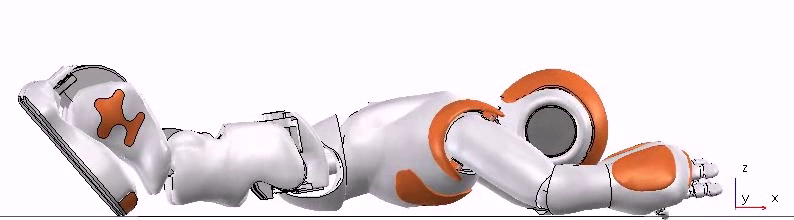
\includegraphics[width=\textwidth]{crawl/vrep/nominal/1.png}
  \caption{This figure shows the Nao humanoid V-REP simulation. 
           The robot is positioned at the initial configuration of the close chain phase
           of the crawl gait.}
  \label{fig:vrep_nao_nom_gait_single_frame1}
\end{figure}

While traversing rough terrain or over small obstacles is one application of a crawl gait,
these experiments were instead designed to show that the robot could access areas with
demanding height constraints. For this, a small table was used whose sides were blocked
with panels down to about $200 mm$ off of the ground. 
Figure \ref{fig:short_ledge_nao_nom_gait_single_frame1} shows the Nao crawling under this table,
with its head almost touching the bottom of the panel. This represents the practical height
constraint that the Nao can satisfy with this gait.

\begin{figure}
  \centering
  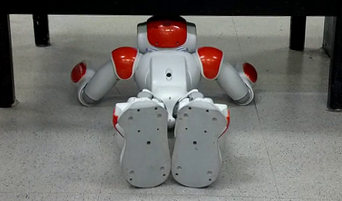
\includegraphics[height=0.35\textheight]{crawl/short_ledge1.png}
  \caption{This figure shows the Nao as it crawls under the table with the low panels.
           The head of the robot can be seen to be nearly touching the panel,
           representing the lowest practical traversable height constraint.}
  \label{fig:short_ledge_nao_nom_gait_single_frame1}
\end{figure}
% Explain that the point of this setup is to show that the crawl gait is very low profile.

\subsection{Gait Parameters} \label{subsec:gait_params}
% Explain the gait and it's parameters.
% Nominal Parameters
As discussed in Chapter \ref{subsec:crawl_closed_chain}, the closed chain phase of the 
Projected Profile crawl gait can be parameterized on the three angles $[\theta_3, \theta_4, \alpha]$.
These three variables are referred to as the gait parameters, or alternatively as the angle triplet.
The nominal angle triplet can be seen in Table \ref{tab:nominal_parameters}. They involve holding
$\theta_3$ and $\theta_4$ constant, while varying $\alpha$ linearly as a function of time.

\begin{table}
  \centering
  \begin{tabularx}{0.5\textwidth}{|l||X|}
    \hline
    \textbf{Gait Parameter} & \textbf{Value}                \\  \hline\hline
    $\theta_3$              &   $16.5^\circ$                \\ 
    $\theta_4$              &   $27.5^\circ$                \\  
    $\alpha$                &   $-30^\circ$ to $-90^\circ$  \\  \hline
  \end{tabularx} 
  
  \caption{Table of gait parameters for the nominal crawl gait. $\theta_3$ and $\theta_4$
           are held constant, while $\alpha$ is linearly decreased in proportion to time.}
  \label{tab:nominal_parameters}
\end{table}

Results using these nominal gait parameters can be seen in Section \ref{sec:nom_crawl_data}.

% Optimal Parameters
% PUT IN HOW MANY ITERATIONS IT TOOK TO FINISH.
% It took like 50 to 80 generations.
% PUT IN HOW MANY ITERATIONS IT TOOK TO KINDA CONVERGE.
% After 10 generations though it was already really close. 

In order to optimize the gait using these parameters, the procedure outlined in Chapter 
\ref{sec:crawl_optimization} was used, modeling the gait parameters as cubic splines.
The Genetic Algorithm in MATLAB's Global Optimization Toolbox was used in conjunction
with the V-REP torque table detailed in Chapter \ref{subsec:crawl_pseudo_static_model}
to generate the optimal spline parameters. 
As the genetic algorithm cannot guarantee finding the global optima for any arbitrary function,
the optimization was executed several times and the best spline parameters were used
in the experiment. Each optimization used 50 to 80 generations to converge on results,
but as can be seen in Figure \ref{fig:ga_generations}, after about 10 generations the
optimization was very near the minima.

\begin{figure}
  \centering
  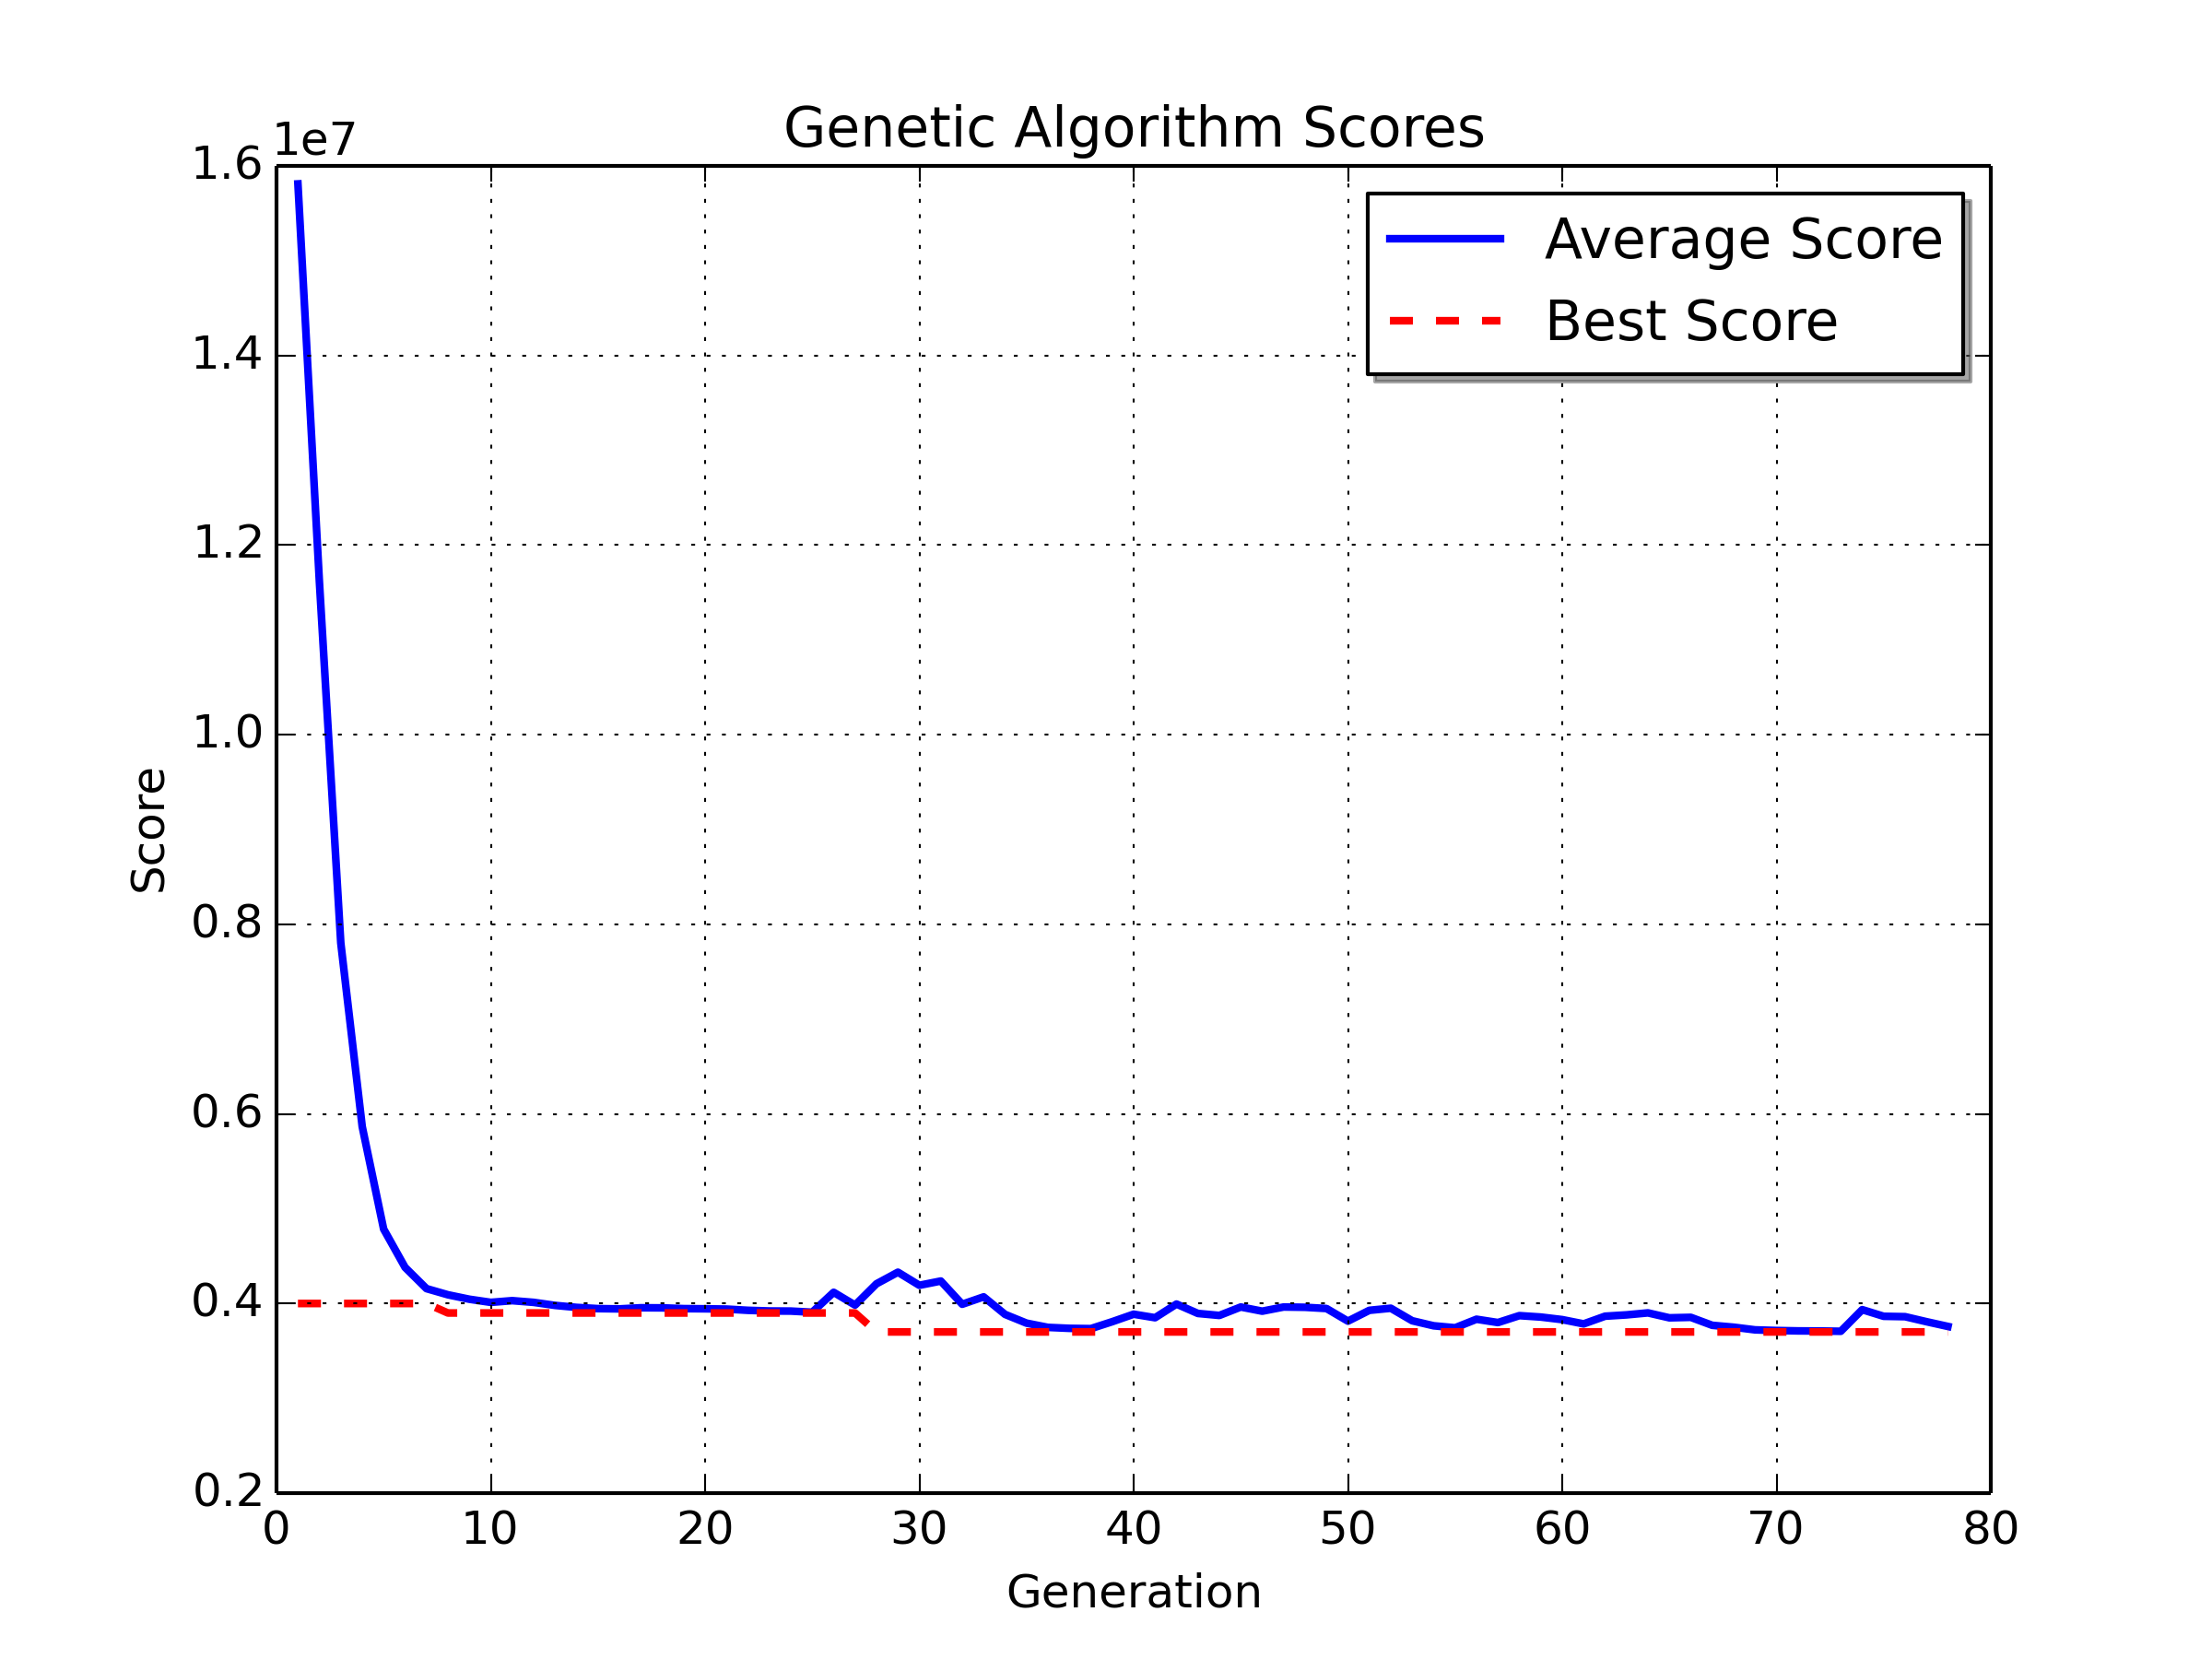
\includegraphics[height=0.35\textheight]{crawl/cost/genetic_alg_scores.png}
  \caption{This figures shows one of the gait parameter optimization trials.
           As the genetic optimization procedure uses multiple childen, the 
           plot shows the average score for the children and the score of the best
           child as the generations progress.}
  \label{fig:ga_generations}
\end{figure}

%%% TABULATE THIS
% specified initial and final values of (\alpha, \theta_3, \theta_4)
% x_init = [-30*pi/180 ; 0.28798  ;   0.47997];

% best x value found after a few runs of the genetic algorithm
% x_best = [-0.2134    1.1570   -1.9898    0.2365    0.0893   -0.3267    1.8796   -0.1365   -1.7434];

% optimized trajectory
% \alpha =   x1_ = x_best(1)*t.^3 + x_best(2)*t.^2 + x_best(3)*t + x_init(1);
% \theta_3 = x2_ = x_best(4)*t.^3 + x_best(5)*t.^2 + x_best(6)*t + x_init(2);
% \theta_4 = x3_ = x_best(7)*t.^3 + x_best(8)*t.^2 + x_best(9)*t + x_init(3);
%%%

Table \ref{tab:optimal_parameters} shows the spine parameters resulting from the
optimization procedure. 
Each gait parameter is now a cubic polynomial which is a function of time $[\theta_3 (t), \theta_4 (t), \alpha (t)]$.
The coefficients from the table are used as $c_3 t^3 + c_2 t^2 + c_1 t + c_0$.
The $c_0$ coefficients are simply the angles corresponding to the starting pose for the closed chain phase
of the gait. The splines are also constrained to end at the final pose for the closed chain phase, which
correspond to the angle triplet of $[0.28798, 0.47997, -1.5710]$ for $[\theta_3, \theta_4, \alpha]$.
The initial and final angle triplets are in radians.

\begin{table}
  \centering
  \begin{tabularx}{0.75\textwidth}{|l|l|l|l|X|}
    \hline
    \textbf{Gait Parameter} & \textbf{$c_3$} & \textbf{$c_2$} & \textbf{$c_1$} & \textbf{$c_0$} \\  \hline\hline
    $\theta_3$              &   0.2365       &  0.0893        & -0.3267        &  0.28798       \\ 
    $\theta_4$              &   1.8796       & -0.1365        & -1.7434        &  0.47997       \\  
    $\alpha$                &  -0.2134       &  1.1570        & -1.9898        &  0.52360       \\  \hline
  \end{tabularx} 
  
  \caption{Table of gait parameter coefficients for the optimal crawl gait. 
           The $c_i$ coefficients are used in the cubic spline 
           $c_3 t^3 + c_2 t^2 + c_1 t + c_0$ to vary the gait parameters as a function of time.
           The $c_0$ coefficients are simply the initial starting angles for each parameter.}
  \label{tab:optimal_parameters}
\end{table}

Figure \ref{fig:optimal_gait_parameters} shows the splines graphically, with the nominal gait parameters
overlaid for comparison. While the optimized parameter trajectory for $\alpha$ is similar to its nominal
trajectory, the trajectories for $\theta_3$ and $\theta_4$ dip significantly, with $\theta_4$ having the
most drastic deviation from the nominal.

\begin{figure}
  \centerline{
    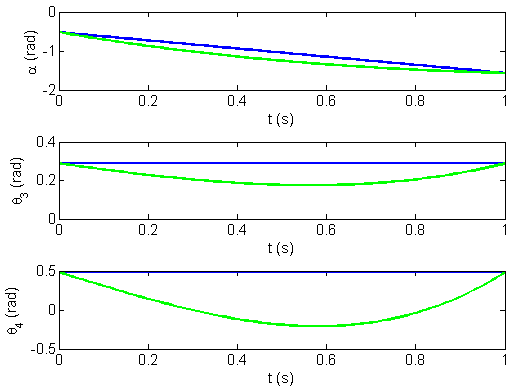
\includegraphics[width=0.75\textwidth]{crawl/cost/ga_cost2_plot1_edit1.png}
  }
  \caption{This figure shows the optimal gait parameter trajectories overlaid onto the nominal
           trajectories. The blue lines represent the nominal trajectories while the green
           lines show the optimal.}
  \label{fig:optimal_gait_parameters}
\end{figure}




\FloatBarrier
\section{Nominal Crawl Gait Data} \label{sec:nom_crawl_data}

% As reviewed in Section \ref{subsec:gait_params}, ...
% This experiment was done using nominal parameters.
% This is basic thing to do.
To test the Projected Profile gait using the nominal parameters reviewed in 
Section \ref{subsec:gait_params}, the gait sequence was first generated in
MATLAB and then simulated in V-REP. Following this the gait was tested on the
Nao by setting it to crawl under a vertically constrained table in two different
experiments. In the first, the robot was set to the initial crawling pose and
placed on the floor in front of the table. The robot then executed the crawling gait.
In the second experiment the robot was programmed to recognise a fiducial marker,
represented by a red circle mounted to the table, and walk to it. 
The robot then moved to a prone posture and crawled under the table. This procedure
is more throughly examined in Section \ref{sec:crawl_exp_setup}. Joint angle and joint
current data was collected during the table experiments and is presented in this section.
These table experiments demonstate the efficacy of the gait to locomote the robot
and the low profile nature of the gait to allow access to vertically constrained spaces.

\subsection{Simulations}
% Here's the MATLAB Projected Profile gait. You can see it moves the mass forward.
% You can see the theta 3 and 4 are held static.
Figure \ref{fig:pp_nom_gait1} shows samples of the closed chain phase of the Projected
Profile gait using the nominal parameters. It shows a simplified kinematic model
representing a projection of the robot onto the saggital plane. The frames show the
model starting in the inital pose, and by linearly increasing the $\alpha$ gait
parameter and holding the $\theta_3$ and $\theta_4$ parameters constant, the model
shifts forward until $\alpha$ has reached its terminal value. This places the model
at the final closed chain pose. It can be seen the highest point of this gait occurs
at about $z = 100 mm$. This model of course does not include the limb thicknesses nor
the head of the Nao, as it only models joint centers. This model was created using MATLAB
and is used to view the results of the gait sequence generation.

\begin{figure}
  \centerline{
    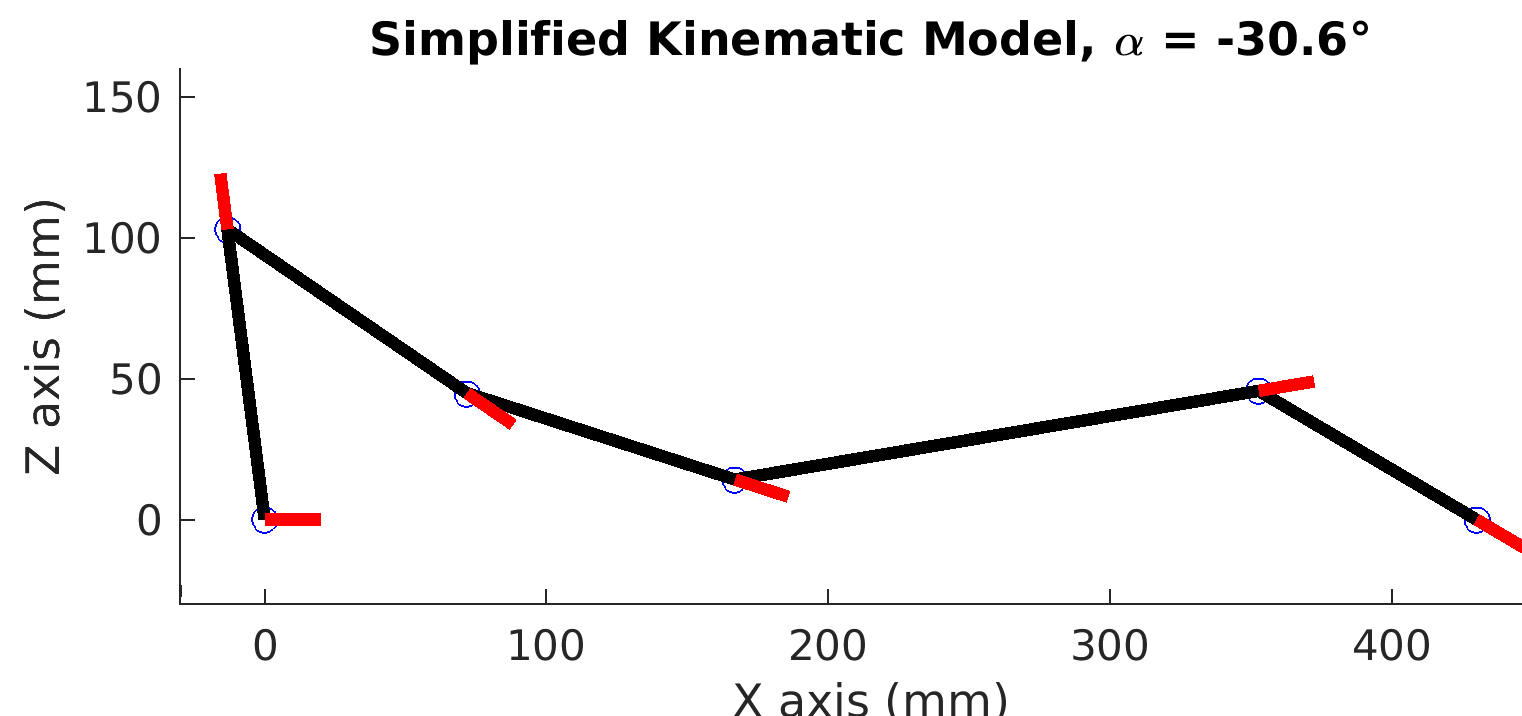
\includegraphics[width=0.5\textwidth]{crawl/pp/nominal/angle30.6_1.png}
    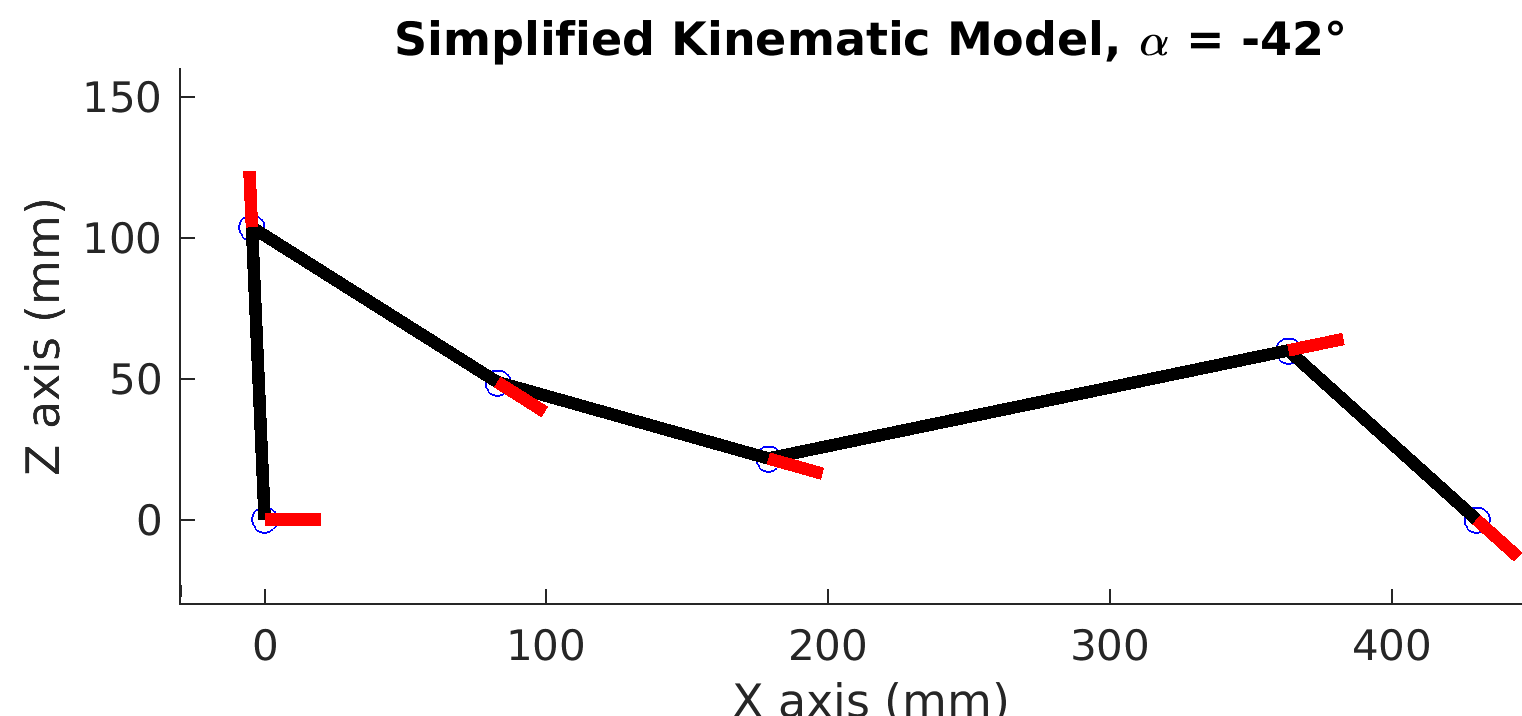
\includegraphics[width=0.5\textwidth]{crawl/pp/nominal/angle42_1.png}
  }
  \centerline{
    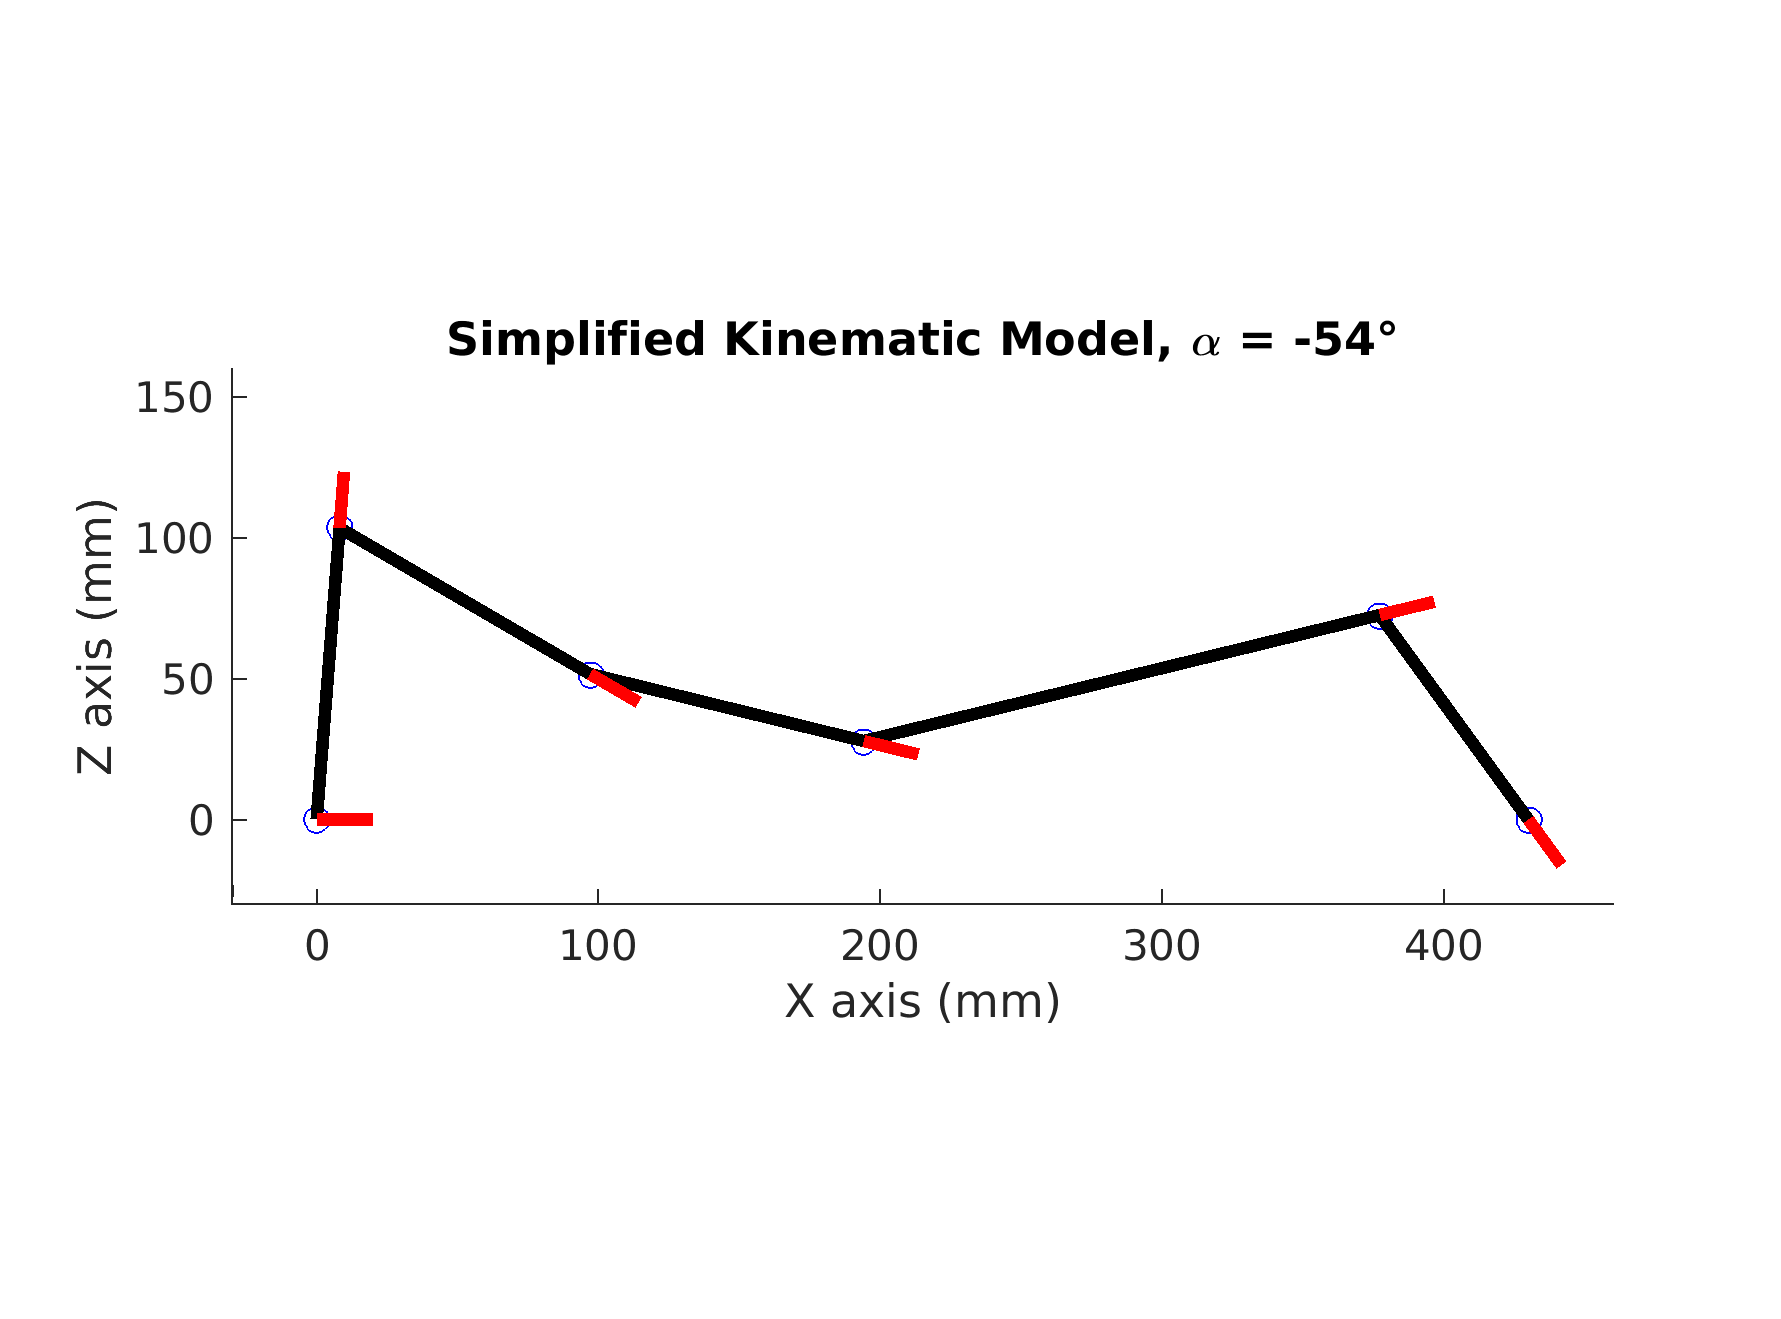
\includegraphics[width=0.5\textwidth]{crawl/pp/nominal/angle54_1.png}
    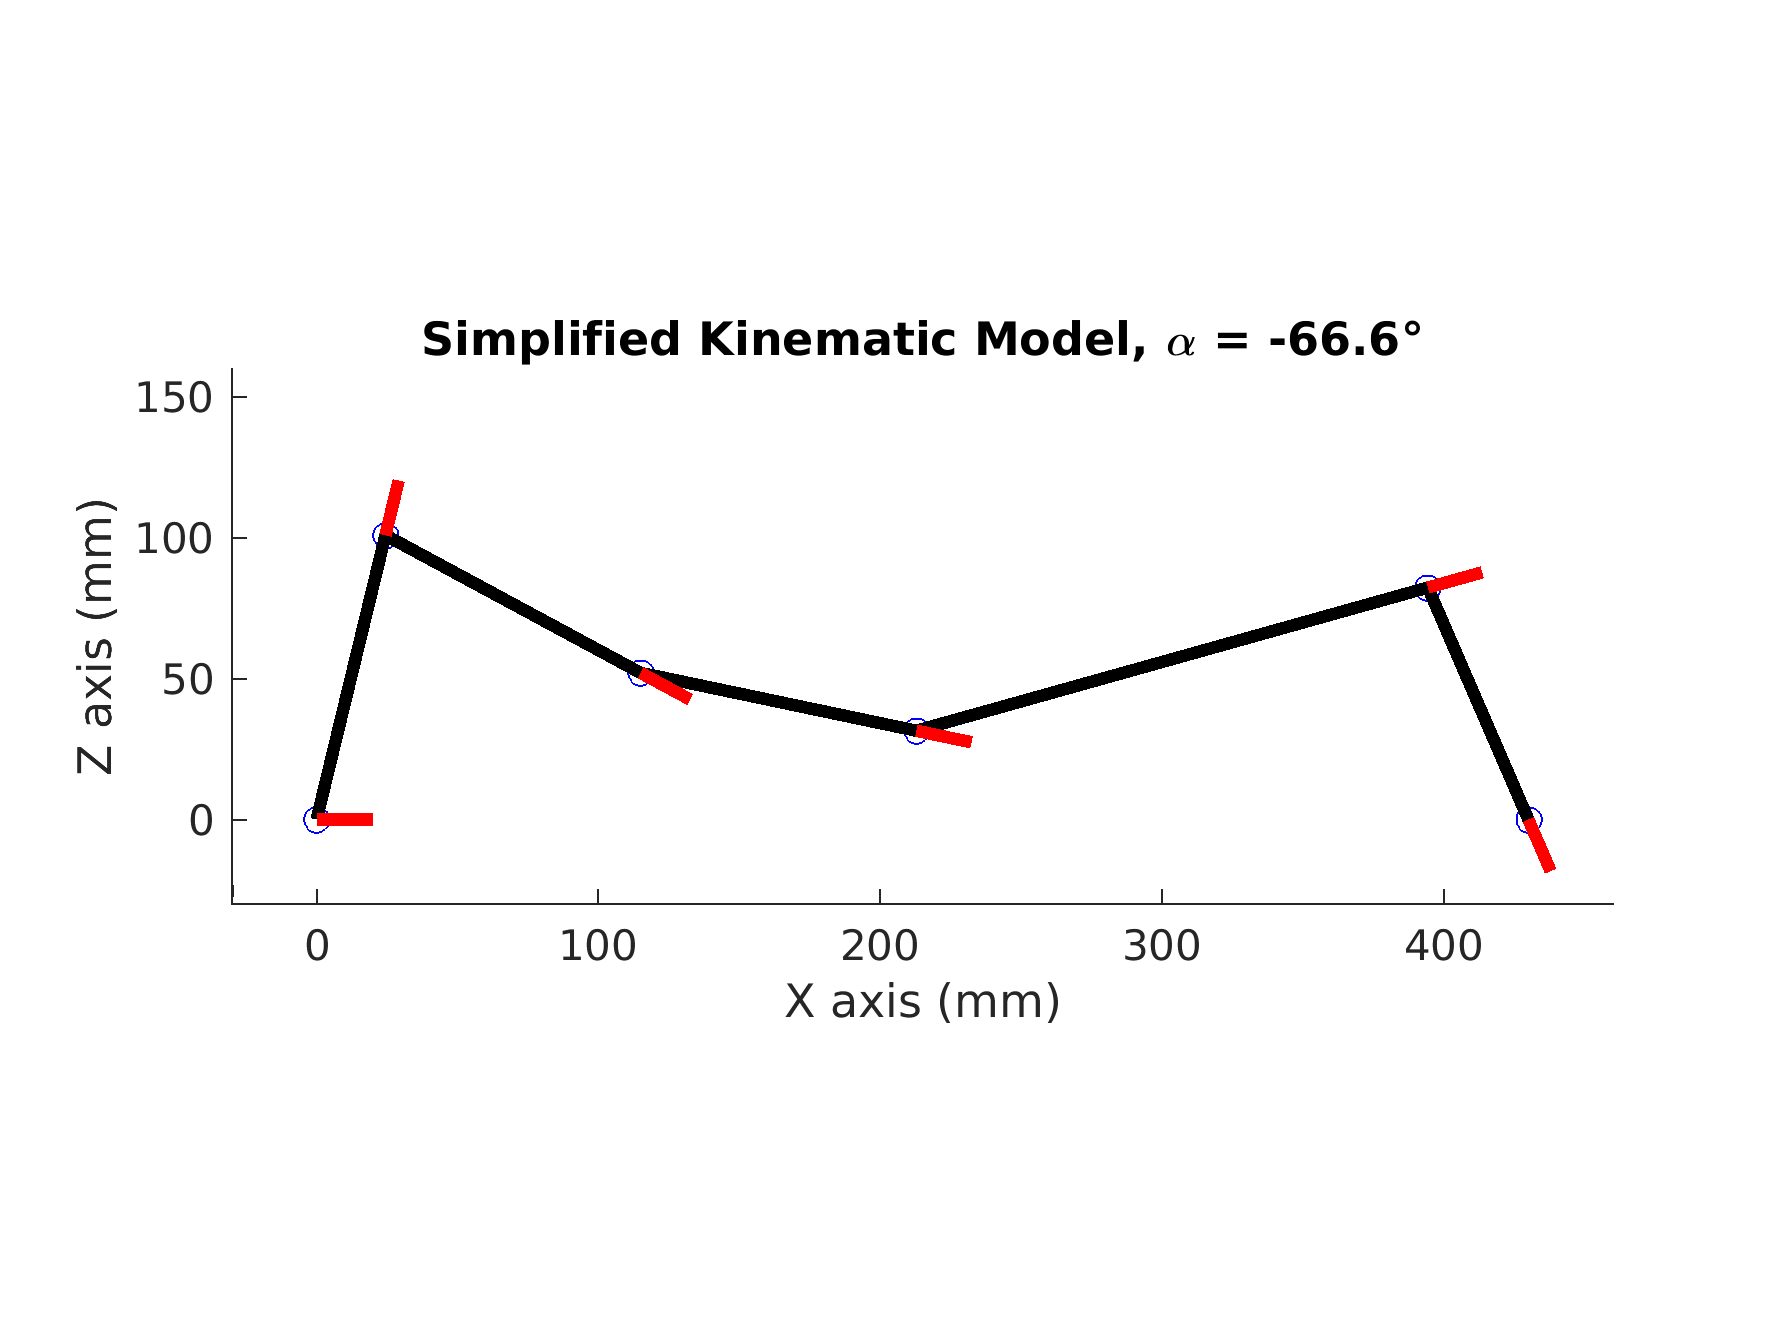
\includegraphics[width=0.5\textwidth]{crawl/pp/nominal/angle66.6_1.png}
  }
  \centerline{
    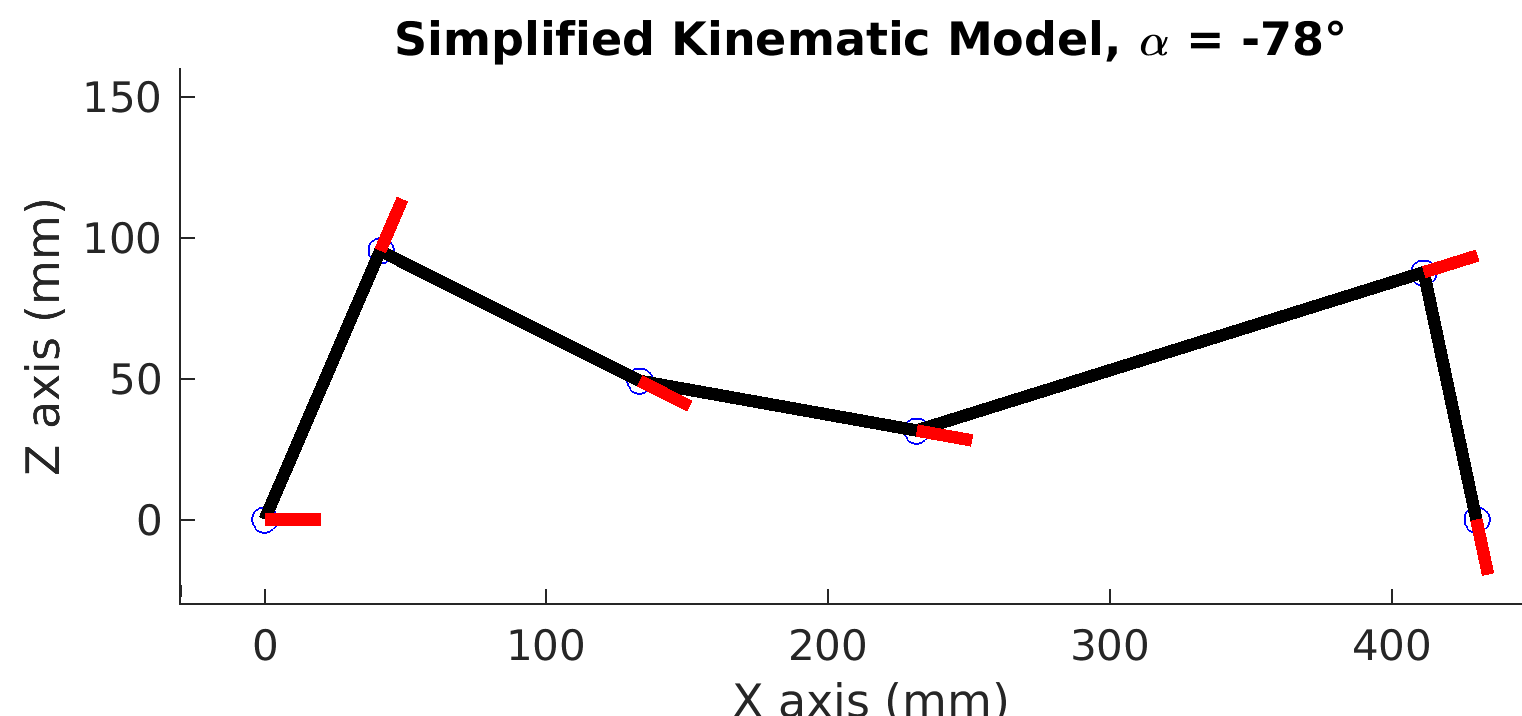
\includegraphics[width=0.5\textwidth]{crawl/pp/nominal/angle78_1.png}
    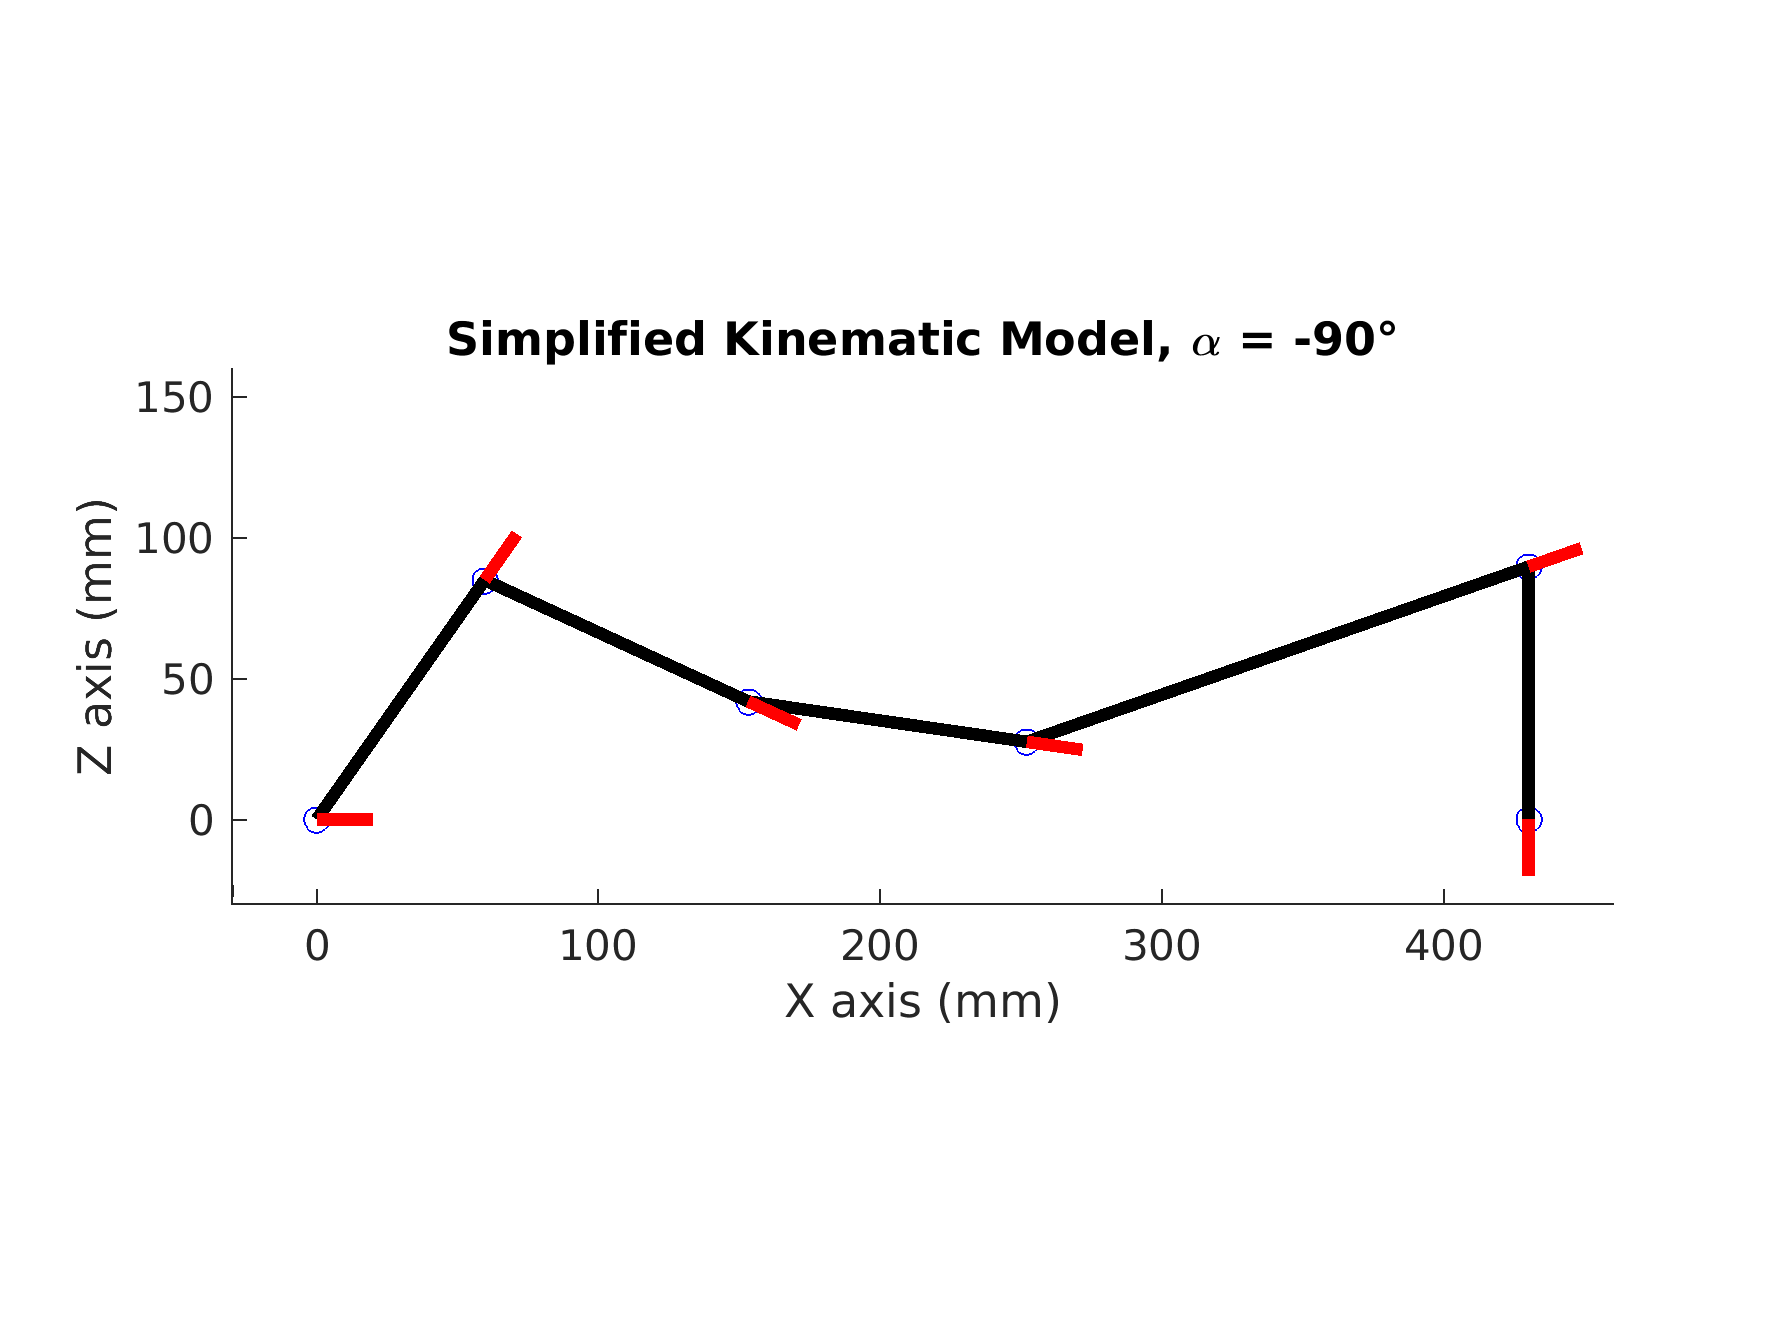
\includegraphics[width=0.5\textwidth]{crawl/pp/nominal/angle90_1.png}
  }
  \caption{This figure shows a simplified kinematic model of the Nao as it executes
           the Projected Profile gait using nominal parameters. The model starts with
           $\alpha = -30^\circ$ and terminates when $\alpha = -90^\circ$.}
  \label{fig:pp_nom_gait1}
\end{figure}

% Here's the V-REP gait. You can see it moves the mass forward.
% The arms are down the whole time.
% You can see the knee and hip are held static.

Once the gait sequence is generated, it is tested using the V-REP simulation of the
Nao humanoid. Figure \ref{fig:vrep_nao_nom_gait1} shows the simulated Nao executing
the closed chain phase of the nominal crawl gait. As with the simplified kinematic
model, the $\alpha$ gait parameter is linearly increased from $-30^\circ$ to $-90^\circ$,
which moves the robot forward. As detailed in Chapter \ref{subsec:nao_kinematics}, the
gait parameters and other constraints are used to position the arms of the robot, as unlike
leg, hip, and shoulder pitch joint which have angles which directly correspond to
joint angles in the simplified kinematic model, the shoulder roll and elbow joints
do not. The head in this simulation can be seen to be the highest part of the robot
throughout the majority of the gait, increasing the minimum value of the allowable
vertical constraint.

\begin{figure}
  \centerline{
    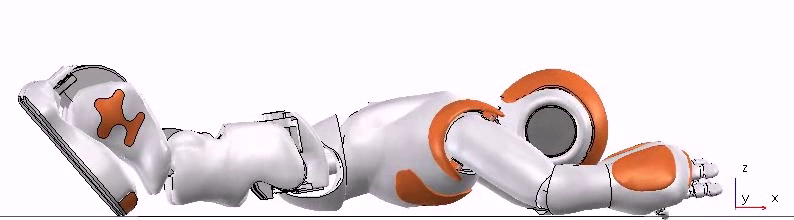
\includegraphics[width=0.5\textwidth]{crawl/vrep/nominal/1.png}
    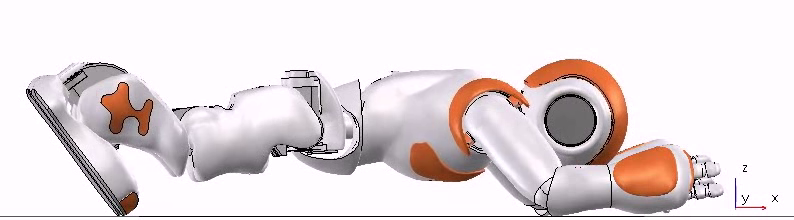
\includegraphics[width=0.5\textwidth]{crawl/vrep/nominal/2.png}
  }
  \centerline{
    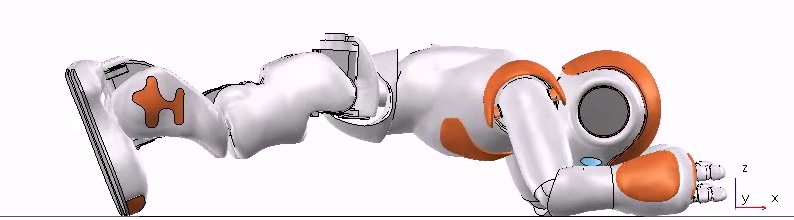
\includegraphics[width=0.5\textwidth]{crawl/vrep/nominal/3.png}
    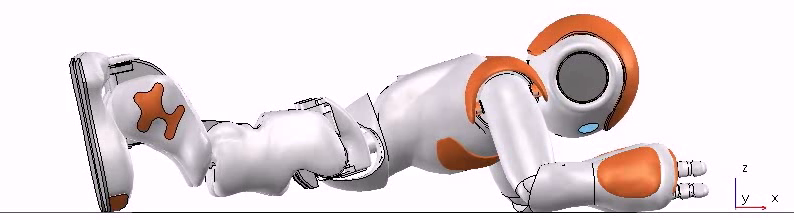
\includegraphics[width=0.5\textwidth]{crawl/vrep/nominal/4.png}
  }
  \centerline{
    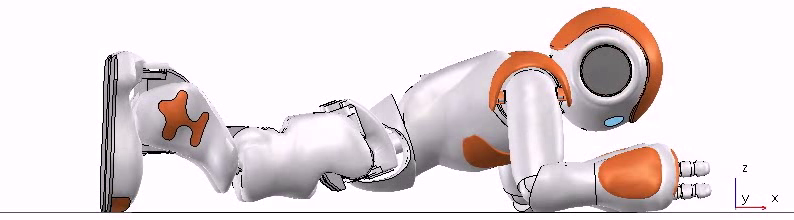
\includegraphics[width=0.5\textwidth]{crawl/vrep/nominal/5.png}
  }
  \caption{BLAH BLAH Simulated Nao with nominal gait.}
  \label{fig:vrep_nao_nom_gait1}
\end{figure}

\subsection{Height Constrained Table}

% Here's the Nao doing the crawl under a little ledge.
% You can see it's really low profile.

Following simulation, the Projected Profile crawl gait using the nominal parameters
was tested on the Nao. Figure \ref{fig:nao_table_exp1_crawl1} shows the initial test of the
robot crawling under the vertically constrained table. The Nao is set to the initial
crawling pose on the floor outside of the table. The robot then executes the crawl
gait for several sequences until the robot is under the table.
For this experiment, the robot executed 9 sequences in 27 seconds. The robot travelled
about 1 body lengths or $610 mm$, equating to a velocity of about $22.6 \frac{mm}{s}$.

% \begin{figure}
%   \centerline{
%     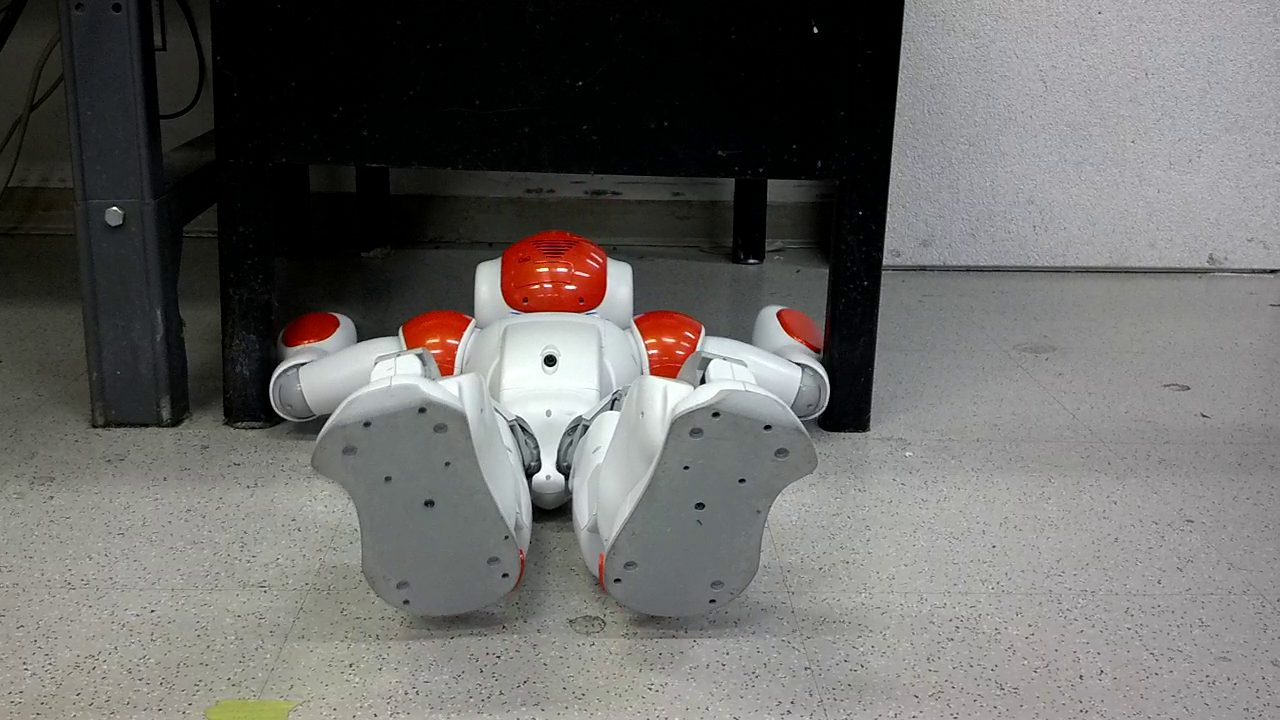
\includegraphics[width=0.25\textwidth]{crawl/under_table/14s.png}
%     \includegraphics[width=0.25\textwidth]{crawl/under_table/18s.png}
%     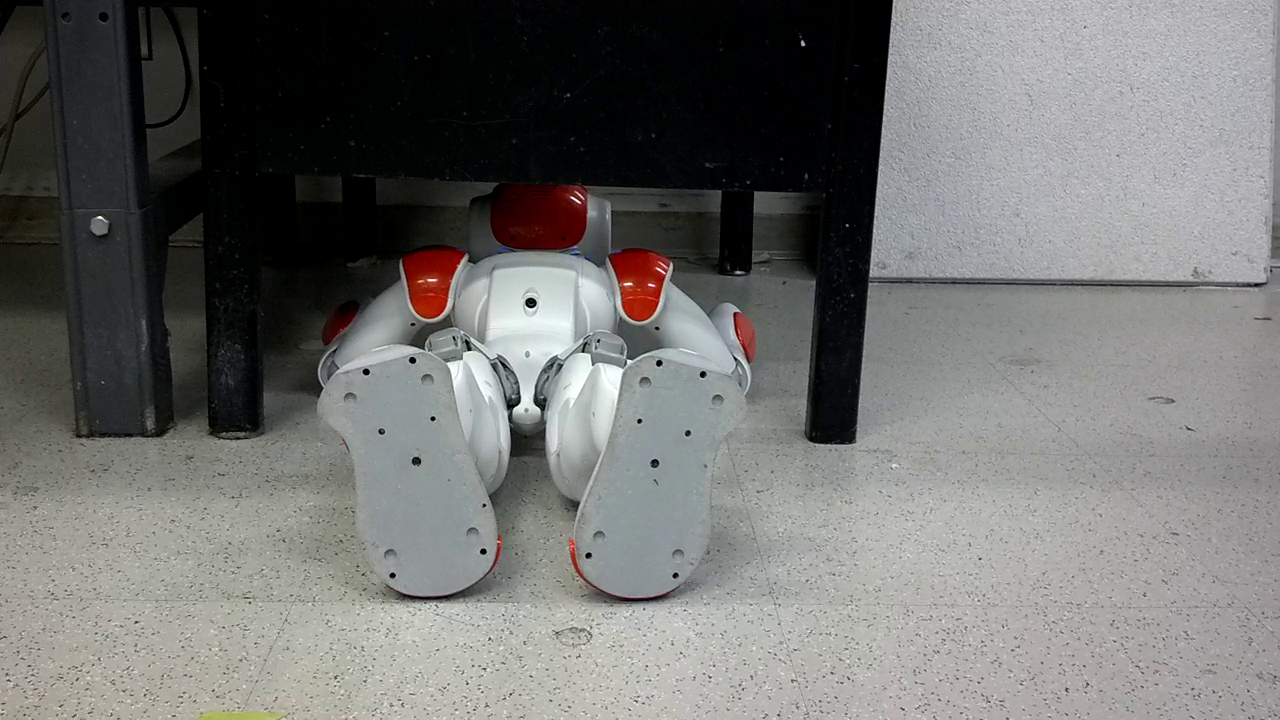
\includegraphics[width=0.25\textwidth]{crawl/under_table/19s.png}
%     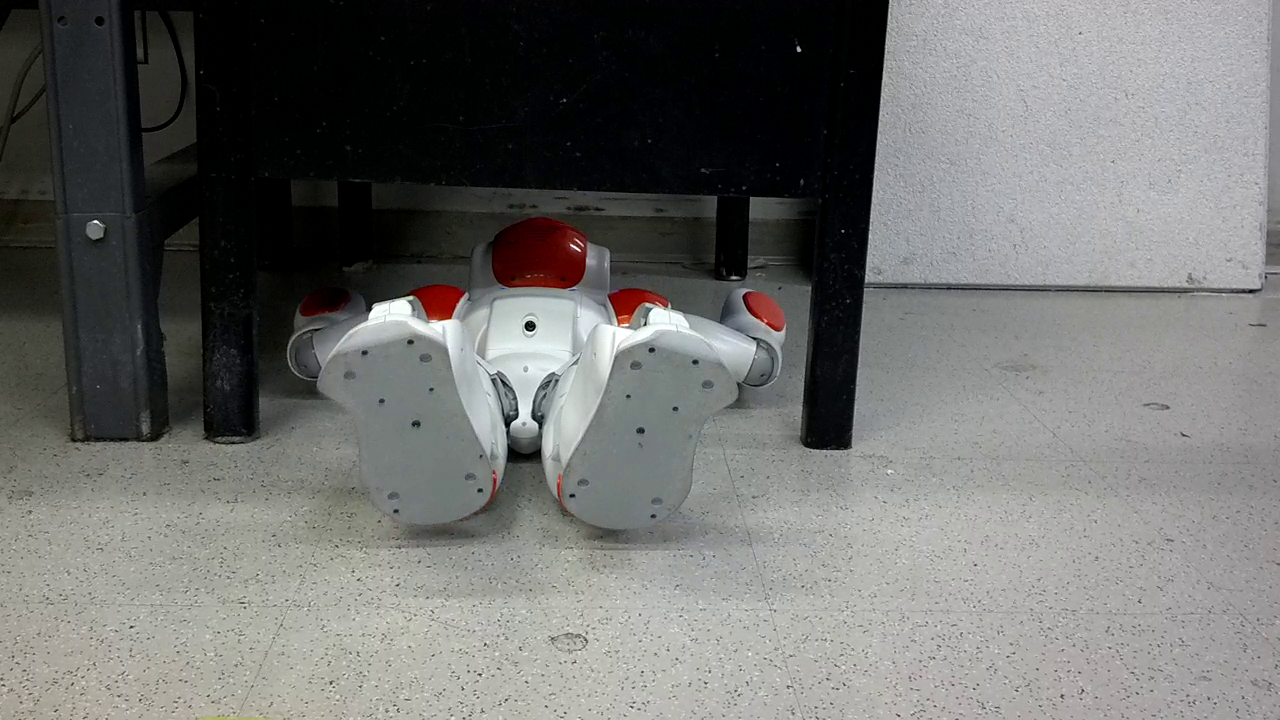
\includegraphics[width=0.25\textwidth]{crawl/under_table/20s.png}
%   }
%   \caption{Low-profile crawling gait for accessing vertically constrained spaces such as under a table.}
%   \label{fig:nao_crawl1}
% \end{figure}

\begin{figure}
  \centerline{
    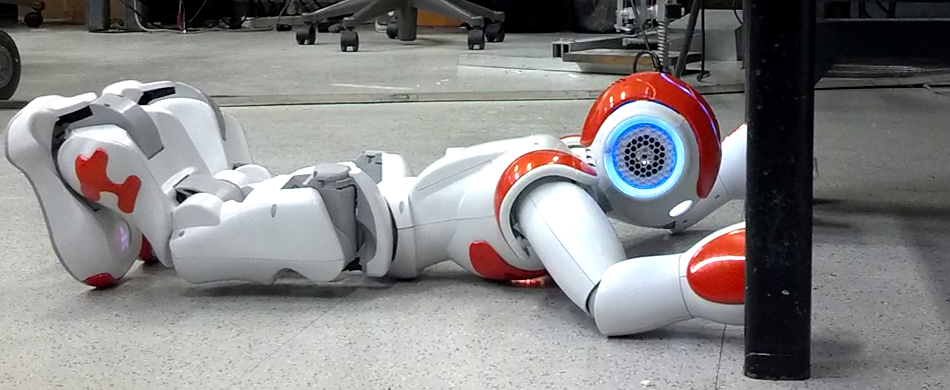
\includegraphics[width=0.33\textwidth]{crawl/under_table/profile_sequence/01.png}
    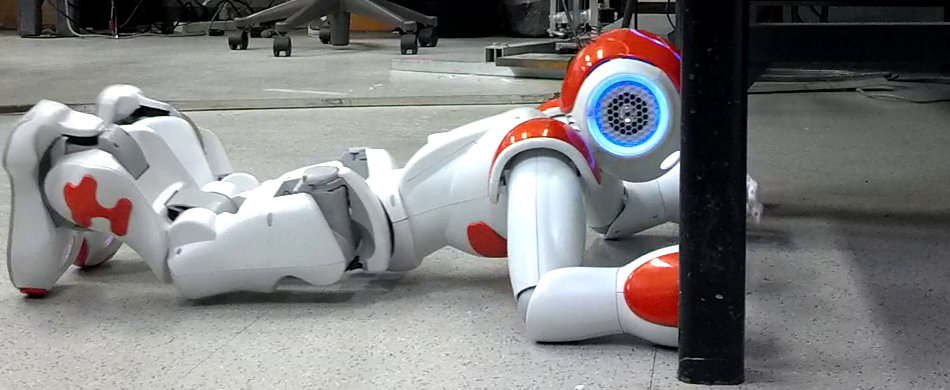
\includegraphics[width=0.33\textwidth]{crawl/under_table/profile_sequence/02.png}
    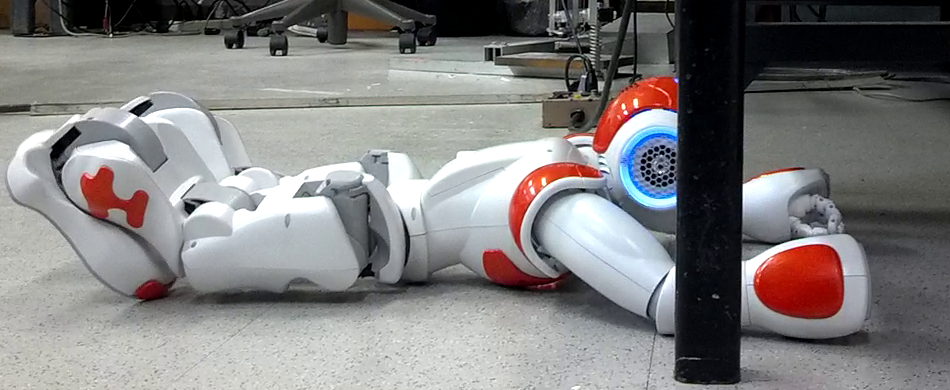
\includegraphics[width=0.33\textwidth]{crawl/under_table/profile_sequence/03.png}
  }
  \vspace*{0.05in}
  \centerline{
    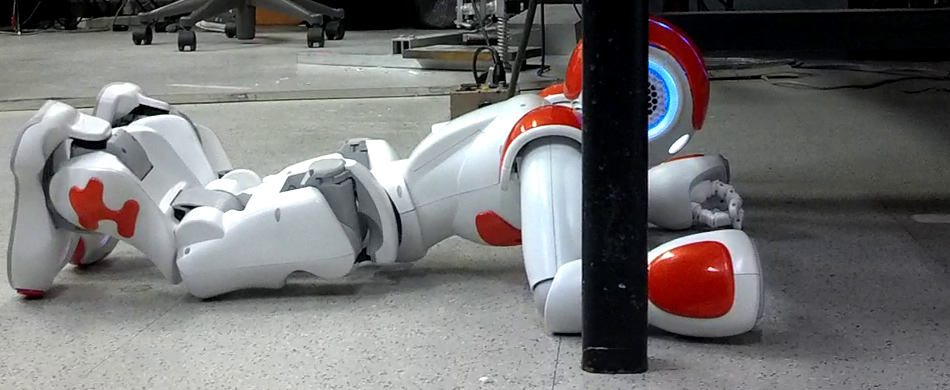
\includegraphics[width=0.33\textwidth]{crawl/under_table/profile_sequence/04.png}
    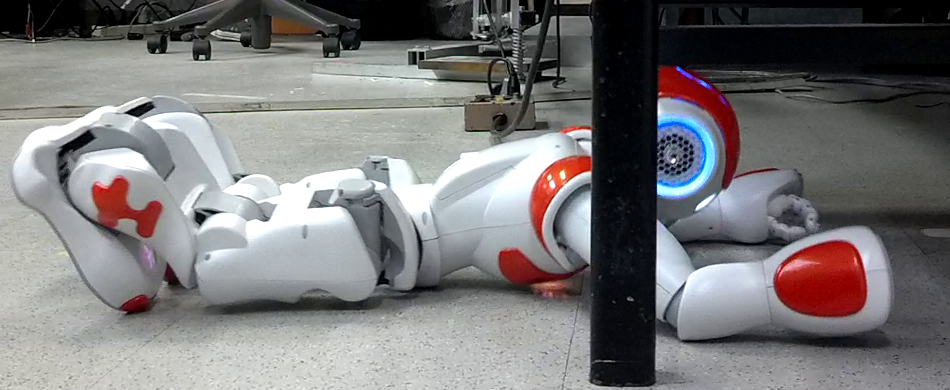
\includegraphics[width=0.33\textwidth]{crawl/under_table/profile_sequence/05.png}
    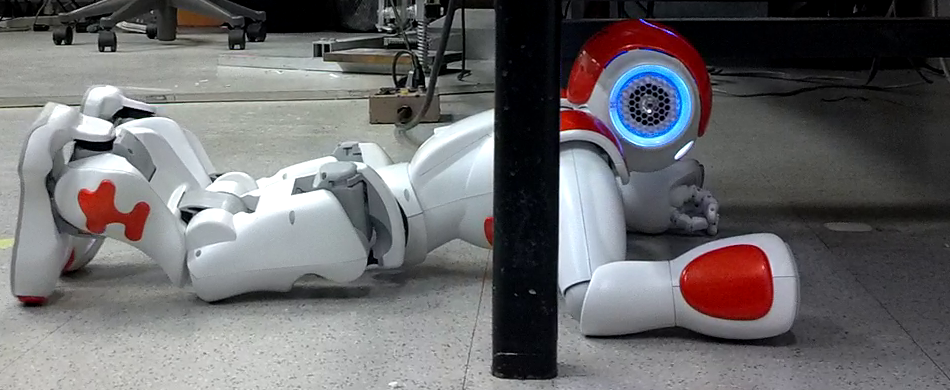
\includegraphics[width=0.33\textwidth]{crawl/under_table/profile_sequence/06.png}
  }
    \vspace*{0.05in}
  \centerline{
    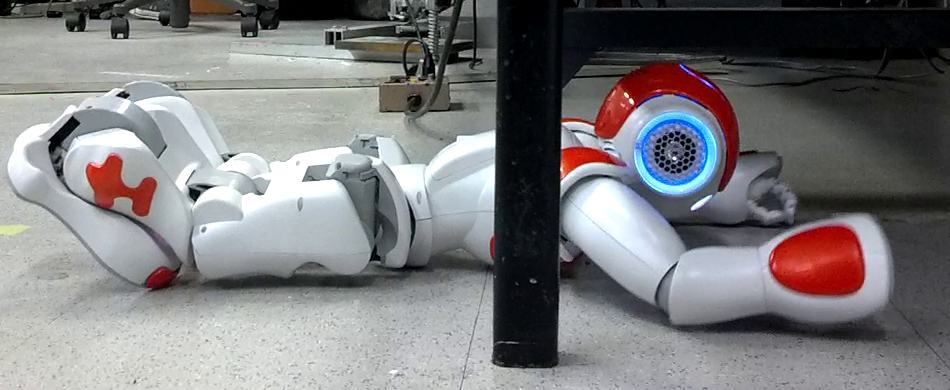
\includegraphics[width=0.33\textwidth]{crawl/under_table/profile_sequence/07.png}
    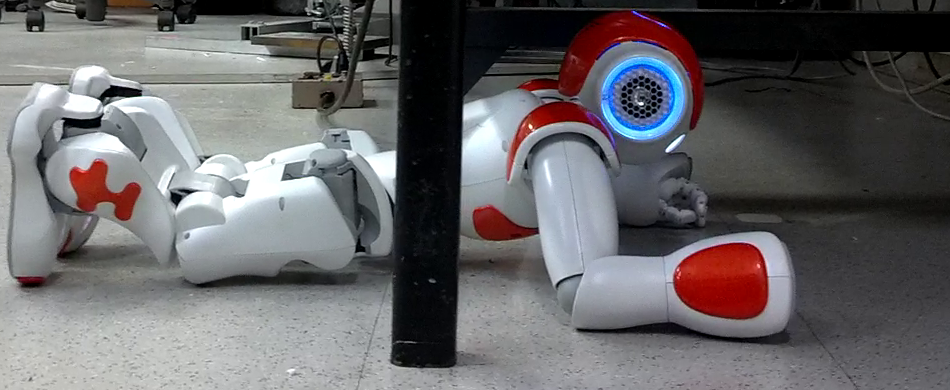
\includegraphics[width=0.33\textwidth]{crawl/under_table/profile_sequence/08.png}
    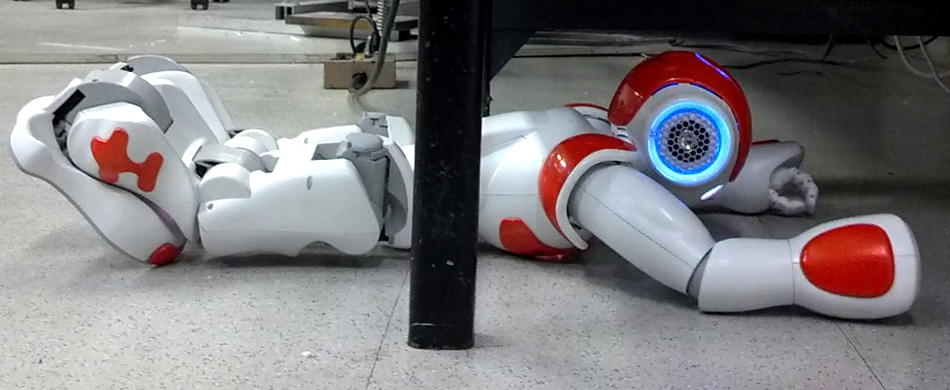
\includegraphics[width=0.33\textwidth]{crawl/under_table/profile_sequence/09.png}
  }
    \vspace*{0.05in}
  \centerline{
    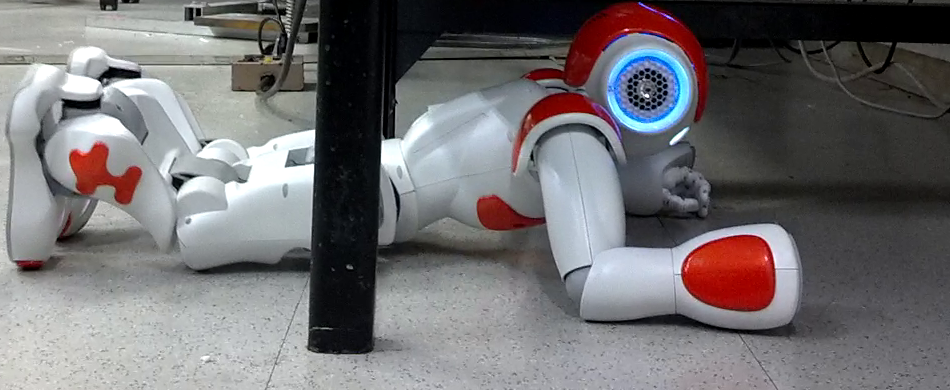
\includegraphics[width=0.33\textwidth]{crawl/under_table/profile_sequence/10.png}
    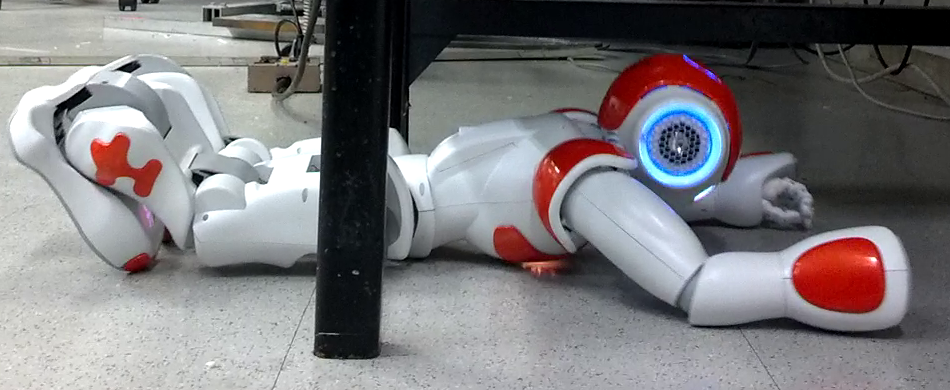
\includegraphics[width=0.33\textwidth]{crawl/under_table/profile_sequence/11.png}
    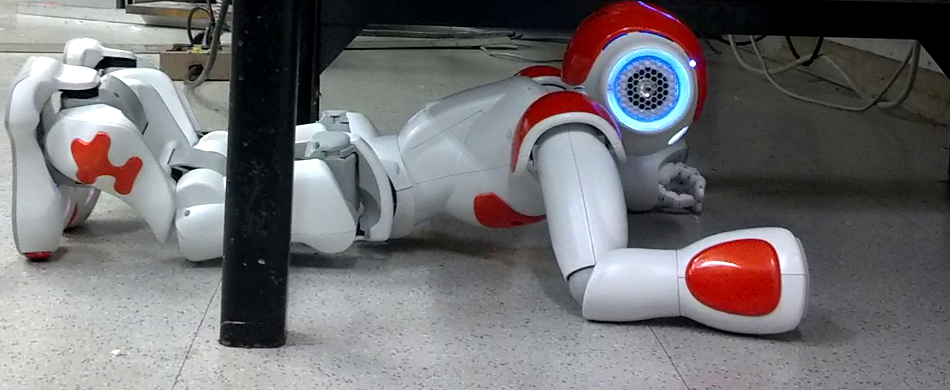
\includegraphics[width=0.33\textwidth]{crawl/under_table/profile_sequence/12.png}
  }
    \vspace*{0.05in}
  \centerline{
    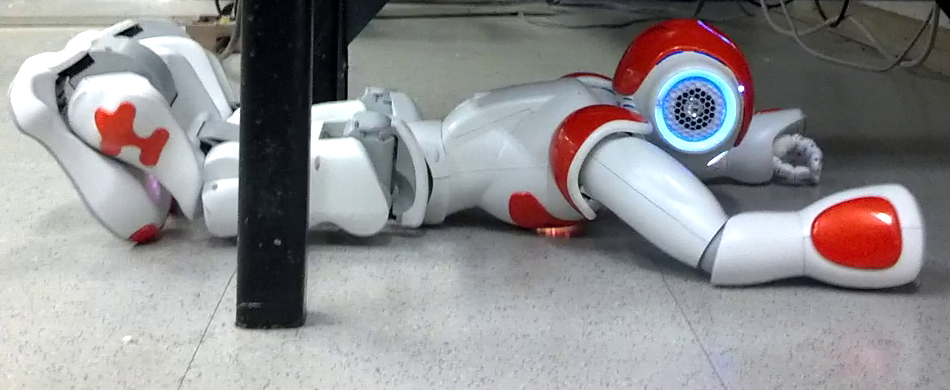
\includegraphics[width=0.33\textwidth]{crawl/under_table/profile_sequence/13.png}
    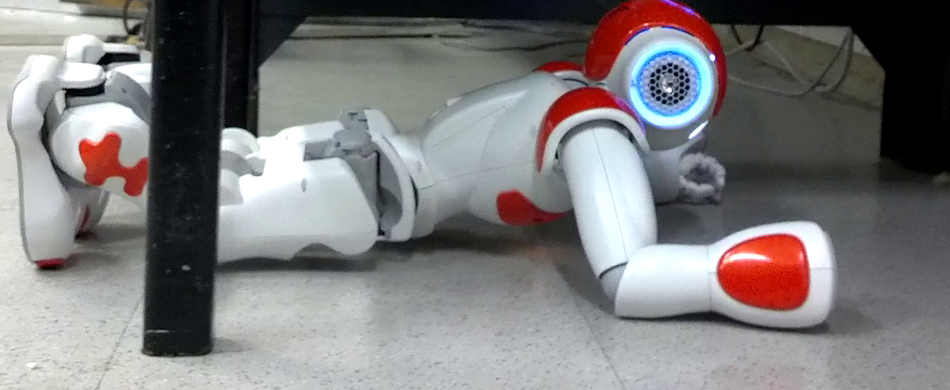
\includegraphics[width=0.33\textwidth]{crawl/under_table/profile_sequence/14.png}
    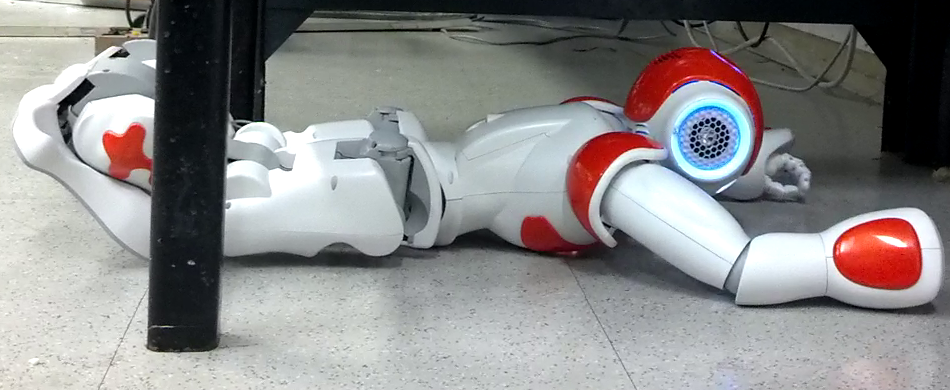
\includegraphics[width=0.33\textwidth]{crawl/under_table/profile_sequence/15.png}
  }
    \vspace*{0.05in}
  \centerline{
    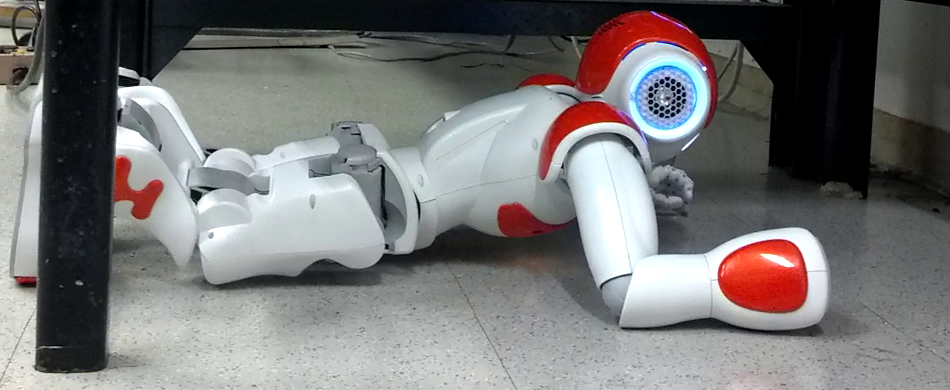
\includegraphics[width=0.33\textwidth]{crawl/under_table/profile_sequence/16.png}
    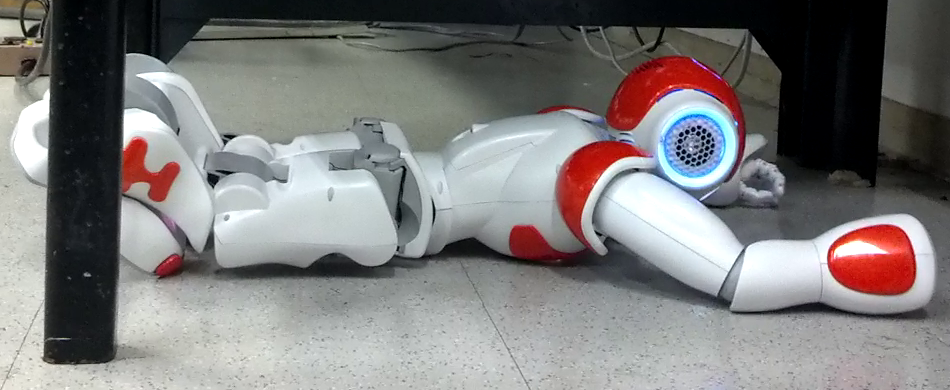
\includegraphics[width=0.33\textwidth]{crawl/under_table/profile_sequence/17.png}
    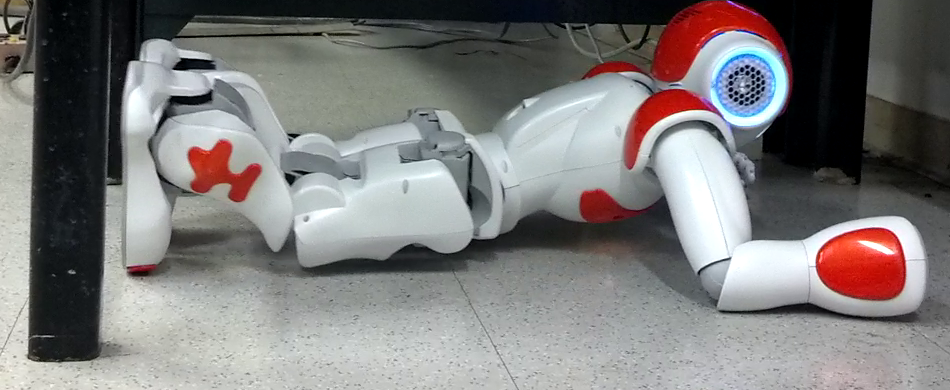
\includegraphics[width=0.33\textwidth]{crawl/under_table/profile_sequence/18.png}
  }
  \caption{This figure shows the Nao crawling under the vertically constrained table.}
  \label{fig:nao_table_exp1_crawl1}
\end{figure}

% Explain that this experiment is a demonstration of the gait being used to perform a task,
% walking somewhere, getting through a crawl space, and coming out the other side.
Figure \ref{fig:nao_table_exp2_crawl1} and \ref{fig:nao_table_exp2_crawl2} show the second
experiment performed with the vertically constrained table. The robot has detected and walked to
the red marker affixed to the table. It then transitions to a prone posture and begins the crawling
sequence. After having crawled to the other side, the robot transitions to a sitting posture.
The ability to transition from posture to posture are provided through the NaoQI API.
For this experiment, the robot executed 25 sequences in 58 seconds. The robot travelled
about 2.75 body lengths or $1,676.4 mm$, equating to a velocity of about $28.9 \frac{mm}{s}$.

\begin{figure}
  \centerline{
    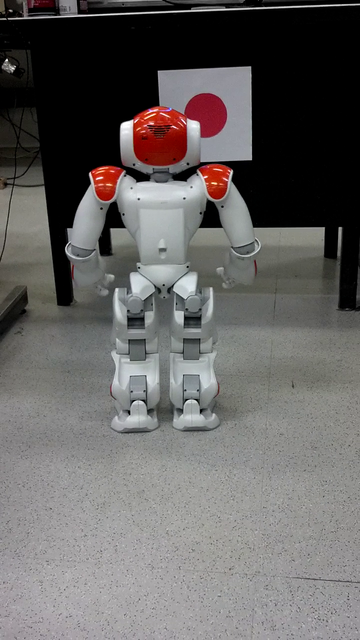
\includegraphics[width=0.2\textwidth]{crawl/walk_to/to/12s.png}
    \includegraphics[width=0.2\textwidth]{crawl/walk_to/to/18s.png}
    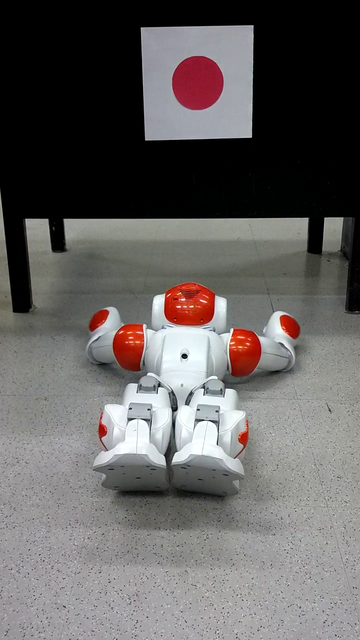
\includegraphics[width=0.2\textwidth]{crawl/walk_to/to/29s.png}
    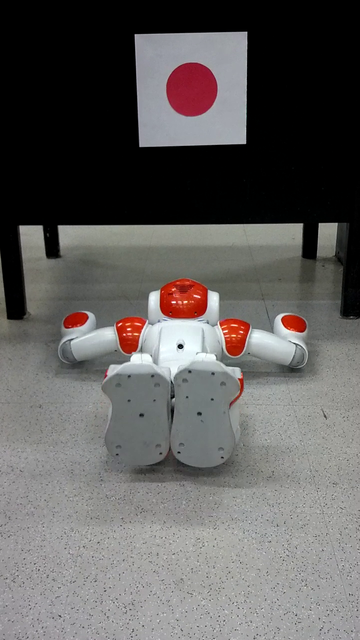
\includegraphics[width=0.2\textwidth]{crawl/walk_to/to/30s_2.png}
    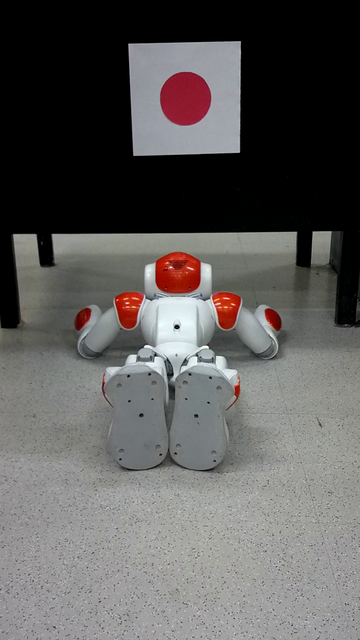
\includegraphics[width=0.2\textwidth]{crawl/walk_to/to/34s.png}
  }
  \vspace*{0.05in}
  \centerline{
    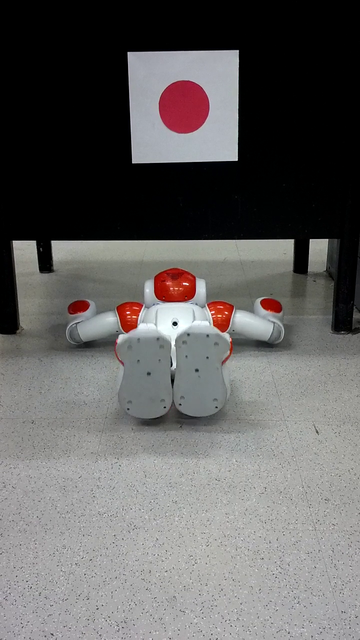
\includegraphics[width=0.2\textwidth]{crawl/walk_to/to/37s.png}
    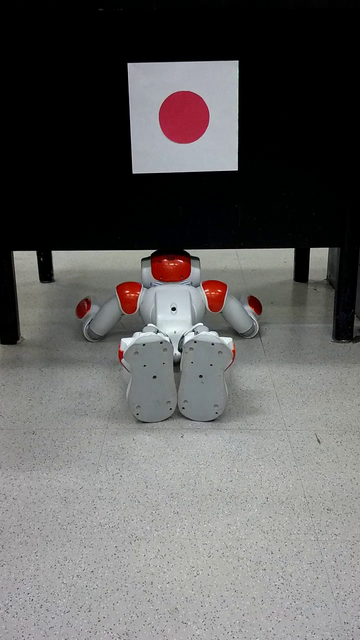
\includegraphics[width=0.2\textwidth]{crawl/walk_to/to/40s.png}
    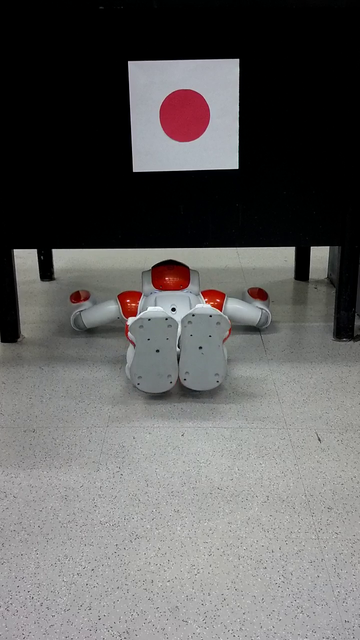
\includegraphics[width=0.2\textwidth]{crawl/walk_to/to/41s.png}
    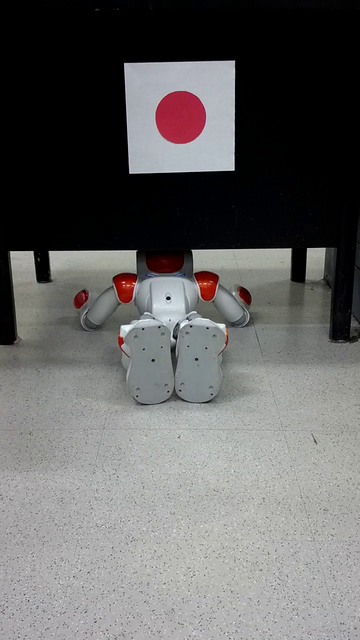
\includegraphics[width=0.2\textwidth]{crawl/walk_to/to/43s.png}
    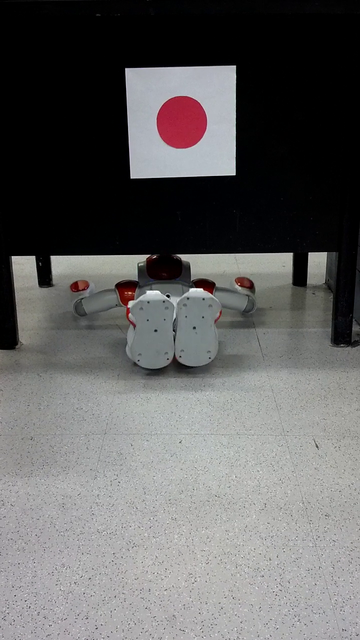
\includegraphics[width=0.2\textwidth]{crawl/walk_to/to/46s.png}
  }
  \caption{BLAH BLAH Approaching and crawling under an obstacle.
           A red dot is used as a marker for the direction in which the robot is commanded to move.
           When the robot approaches below a specified distance threshold from the obstacle,
           the crouch-down and crawl gait sequence is initiated.}
  \label{fig:nao_table_exp2_crawl1}
\end{figure}

\begin{figure}
  \centerline{
    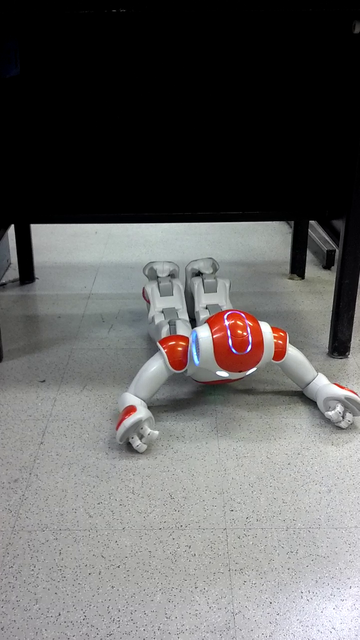
\includegraphics[width=0.2\textwidth]{crawl/walk_to/from/8s.png}
    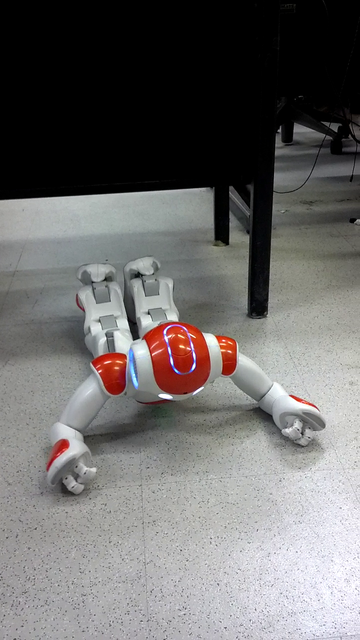
\includegraphics[width=0.2\textwidth]{crawl/walk_to/from/15s.png}
    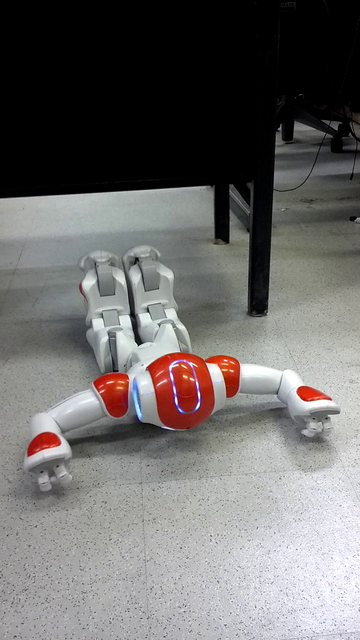
\includegraphics[width=0.2\textwidth]{crawl/walk_to/from/16s.png}
    \includegraphics[width=0.2\textwidth]{crawl/walk_to/from/17s.png}
    \includegraphics[width=0.2\textwidth]{crawl/walk_to/from/18s.png}
  }
  \vspace*{0.05in}
  \centerline{
    \includegraphics[width=0.2\textwidth]{crawl/walk_to/from/24s.png}
    \includegraphics[width=0.2\textwidth]{crawl/walk_to/from/30s.png}
    \includegraphics[width=0.2\textwidth]{crawl/walk_to/from/32s.png}
    \includegraphics[width=0.2\textwidth]{crawl/walk_to/from/35s.png}
    \includegraphics[width=0.2\textwidth]{crawl/walk_to/from/37s.png}
  }
  \caption{BLAH BLAH Crawling under an obstacle and transitioning back to stand posture.}
  \label{fig:nao_table_exp2_crawl2}
\end{figure}

\subsection{Joint Data}
Here is a plot of the joint angles of the gait, showing its periodicity.

\begin{figure}
  \centerline{
    \includegraphics[width=0.5\textwidth]{crawl/joint_angles/LeftArmJointAngles.png}
    \includegraphics[width=0.5\textwidth]{crawl/joint_angles/LeftLegJointAngles.png}
  }
  \caption{Measured motor joint angles during multiple iterations of the periodic crawling gait.
           While the crawling gait is laterally symmetric, the asymmetry in measured angles is due to the
           definitions of the robot frame and joint frame in the NAO API, which essentially forms a mirror
           asymmetry between the left and right joints.}
  \label{fig:nao_joint_angles1}
\end{figure}

This is a full plot of the entire sequence, from walking, to crawling, to walking.

\begin{figure}
  \centerline{
    \includegraphics[width=0.5\textwidth]{crawl/joint_angles_long_sequence/LeftArmJointAngles_longSequence.png}
    \includegraphics[width=0.5\textwidth]{crawl/joint_angles_long_sequence/LeftLegJointAngles_longSequence.png}
  }
  \caption{Measured joint angles for a sequence of transitioning from standing to crouch to crawling,
           crawling under a table, and then returning to crouch.}
  \label{fig:nao_joint_angles_long_seq}
\end{figure}

This plot shows the current draws of the arm and leg joints.
There are some distinct patterns, but is hard to relate torques directly.

\begin{figure}
  \centerline{
    \includegraphics[width=0.5\textwidth]{crawl/current_draws/LeftArmCurrentDraw.png}
    \includegraphics[width=0.5\textwidth]{crawl/current_draws/LeftLegCurrentDraw.png}
  }
  \caption{Measured motor current draws during multiple iterations of the periodic crawling gait.}
  \label{fig:nao_currents}
\end{figure}




\FloatBarrier
\section{Optimized Crawl Gait Data} \label{sec:opt_crawl_data}

This time, we optimized the gait. Here's what happened.

\subsection{Optimization Cost}
These plots show the theoretical optimization costs of the nominal and optimized
triplet parameters. 



\subsection{Simulations}

Here's the MATLAB simulation. The theta 3 and 4 are doing different things.

\begin{figure}
  \centerline{
    \includegraphics[width=0.5\textwidth]{crawl/pp/optimal/angle30_1.png}
    \includegraphics[width=0.5\textwidth]{crawl/pp/optimal/angle42.7474_1.png}
  }
  \centerline{
    \includegraphics[width=0.5\textwidth]{crawl/pp/optimal/angle54.5496_1.png}
    \includegraphics[width=0.5\textwidth]{crawl/pp/optimal/angle66.4421_1.png}
  }
  \centerline{
    \includegraphics[width=0.5\textwidth]{crawl/pp/optimal/angle78.1161_1.png}
    \includegraphics[width=0.5\textwidth]{crawl/pp/optimal/angle89.9428_1.png}
  }
  \caption{BLAH BLAH Projected Profile Nao with optimal gait.}
  \label{fig:pp_opt_gait1}
\end{figure}

Here's the V-REP simulation. The knees and hips are doing different things.
The arms are down the whole time.

\begin{figure}
  \centerline{
    \includegraphics[width=0.5\textwidth]{crawl/vrep/optimized/1.png}
    \includegraphics[width=0.5\textwidth]{crawl/vrep/optimized/2.png}
  }
  \centerline{
    \includegraphics[width=0.5\textwidth]{crawl/vrep/optimized/3.png}
    \includegraphics[width=0.5\textwidth]{crawl/vrep/optimized/4.png}
  }
  \centerline{
    \includegraphics[width=0.5\textwidth]{crawl/vrep/optimized/5.png}
  }
  \caption{BLAH BLAH Simulated Nao with optimized gait.}
  \label{fig:vrep_nao_opt_gait1}
\end{figure}

\subsection{Joint Torque Data} \label{subsec:opt_joint_torque_data}

Ok, so now, how does it do with these new optimizations?
We use the V-REP here instead of the currents from the robot because they are easier to interpret.

Here's the nominal and optimal joint data overlaid for each joint.
It ranges, but you can kinda see the optimal ones look kinda like a compressed version of the
nominal ones.

\begin{figure}
  \centerline{
    \includegraphics[width=\textwidth]{crawl/torques/trimmed/joint2_3_torques.png}
  }
  \centerline{
    \includegraphics[width=\textwidth]{crawl/torques/trimmed/joint4_5_torques.png}
  }
  \caption{BLAH BLAH Simulated joint torques for the different times. Nominal and optimized.}
  \label{fig:vrep_joint_torques_by_joint1}
\end{figure}

Here's the nominal and optimal joint data, side by side, on a duration basis.
You can kinda see the compressions. You can also see that the short ones look similar,
but the longer ones don't.

\begin{figure}
  \centerline{
    \includegraphics[width=0.5\textwidth]{crawl/torques/nom_torques_duration_1.0_1.png}
    \includegraphics[width=0.5\textwidth]{crawl/torques/opt_torques_duration_1.0_1.png}
  }
  \centerline{
    \includegraphics[width=0.5\textwidth]{crawl/torques/nom_torques_duration_5.0_1.png}
    \includegraphics[width=0.5\textwidth]{crawl/torques/opt_torques_duration_5.0_1.png}
  }
  \centerline{
    \includegraphics[width=0.5\textwidth]{crawl/torques/nom_torques_duration_10.0_1.png}
    \includegraphics[width=0.5\textwidth]{crawl/torques/opt_torques_duration_10.0_1.png}
  }
  \caption{BLAH BLAH Simulated joint torques for the different times. Nominal and optimized.}
  \label{fig:vrep_joint_torques_by_duration1}
\end{figure}

Actually summing up the costs you can see there's a difference between the two and the optimal
one is always lower cost.
Percentagewise, the 7 second gait had the biggest difference, but I'd say that anything after
7 seconds has probably converges and takes the most advantage of the optimization.
These costs are for straight sum of torques. They're not weighted.

\begin{figure}
  \includegraphics[width=0.5\textwidth]{crawl/cost/gait_cost_duration1.png}
  \includegraphics[width=0.5\textwidth]{crawl/cost/cost_imp_duration1.png}
  \caption{BLAH BLAH Things about gait cost comparisons.}
  \label{fig:cost_duration1}
\end{figure}


